% Lines starting with a percent sign (%) are comments. LaTeX will
% not process those lines. Similarly, everything after a percent
% sign in a line is considered a comment. To produce a percent sign
% in the output, write \% (backslash followed by the percent sign).
% ==================================================================
% Usage instructions:
% ------------------------------------------------------------------
% The file is heavily commented so that you know what the various
% commands do. Feel free to remove any comments you don't need from
% your own copy. When redistributing the example thesis file, please
% retain all the comments for the benefit of other thesis writers! 
% ==================================================================
% Compilation instructions:
% ------------------------------------------------------------------
% Use pdflatex to compile! Input images are expected as PDF files.
% Example compilation: 
% ------------------------------------------------------------------
% > pdflatex thesis-example.tex
% > bibtex thesis-example
% > pdflatex thesis-example.tex 
% > pdflatex thesis-example.tex
% ------------------------------------------------------------------
% You need to run pdflatex multiple times so that all the cross-references
% are fixed. pdflatex will tell you if you need to re-run it (a warning
% will be issued)
% ------------------------------------------------------------------
% Compilation has been tested to work in ukk.cs.hut.fi and kosh.hut.fi
% - if you have problems of missing .sty -files, then the local LaTeX
% environment does not have all the required packages installed.
% For example, when compiling in vipunen.hut.fi, you get an error that
% tikz.sty is missing - in this case you must either compile somewhere
% else, or you cannot use TikZ graphics in your thesis and must therefore
% remove or comment out the tikz package and all the tikz definitions.
% ------------------------------------------------------------------

% General information
% ==================================================================
% Package documentation:
%
% The comments often refer to package documentation. (Almost) all LaTeX
% packages have documentation accompanying them, so you can read the
% package documentation for further information. When a package 'xxx' is
% installed to your local LaTeX environment (the document compiles
% when you have \usepackage{xxx} and LaTeX does not complain), you can
% find the documentation somewhere in the local LaTeX texmf directory
% hierarchy. In ukk.cs.hut.fi, this is /usr/texlive/2008/texmf-dist,
% and the documentation for the titlesec package (for example) can be
% found at /usr/texlive/2008/texmf-dist/doc/latex/titlesec/titlesec.pdf.
% Most often the documentation is located as a PDF file in
% /usr/texlive/2008/texmf-dist/doc/latex/xxx, where xxx is the package name;
% however, documentation for TikZ is in
% /usr/texlive/2008/texmf-dist/doc/latex/generic/pgf/pgfmanual.pdf
% (this is because TikZ is a front-end for PGF, which is meant to be a
% generic portable graphics format for LaTeX).
% You can try to look for the package manual using the ``find'' shell
% command in Linux machines; the find databases are up-to-date at least
% in ukk.cs.hut.fi. Just type ``find xxx'', where xxx is the package
% name, and you should find a documentation file.
% Note that in some packages, the documentation is in the DVI file
% format. In this case, you can copy the DVI file to your home directory,
% and convert it to PDF with the dvipdfm command (or you can read the
% DVI file directly with a DVI viewer).
%
% If you can't find the documentation for a package, just try Googling
% for ``latex packagename''; most often you can get a direct link to the
% package manual in PDF format.
% ------------------------------------------------------------------


% Document class for the thesis is report
% ------------------------------------------------------------------
% You can change this but do so at your own risk - it may break other things.
% Note that the option pdftext is used for pdflatex; there is no
% pdflatex option.
% ------------------------------------------------------------------
\documentclass[12pt,a4paper,oneside,pdftex]{report}

% The input files (tex files) are encoded with the latin-1 encoding
% (ISO-8859-1 works). Change the latin1-option if you use UTF8
% (at some point LaTeX did not work with UTF8, but I'm not sure
% what the current situation is)
\usepackage[utf8]{inputenc}
% OT1 font encoding seems to work better than T1. Check the rendered
% PDF file to see if the fonts are encoded properly as vectors (instead
% of rendered bitmaps). You can do this by zooming very close to any letter
% - if the letter is shown pixelated, you should change this setting
% (try commenting out the entire line, for example).
\usepackage[OT1]{fontenc}
% The babel package provides hyphenating instructions for LaTeX. Give
% the languages you wish to use in your thesis as options to the babel
% package (as shown below). You can remove any language you are not
% going to use.
% Examples of valid language codes: english (or USenglish), british,
% finnish, swedish; and so on.
\usepackage[finnish,swedish,english]{babel}
\usepackage[sf]{titlesec}

\usepackage{float}

% Font selection
% ------------------------------------------------------------------
% The default LaTeX font is a very good font for rendering your
% thesis. It is a very professional font, which will always be
% accepted.
% If you, however, wish to spicen up your thesis, you can try out
% these font variants by uncommenting one of the following lines
% (or by finding another font package). The fonts shown here are
% all fonts that you could use in your thesis (not too silly).
% Changing the font causes the layouts to shift a bit; you many
% need to manually adjust some layouts. Check the warning messages
% LaTeX gives you.
% ------------------------------------------------------------------
% To find another font, check out the font catalogue from
% http://www.tug.dk/FontCatalogue/mathfonts.html
% This link points to the list of fonts that support maths, but
% that's a fairly important point for master's theses.
% ------------------------------------------------------------------
% <rant>
% Remember, there is no excuse to use Comic Sans, ever, in any
% situation! (Well, maybe in speech bubbles in comics, but there
% are better options for those too)
% </rant>

%\usepackage{tgcursor}
%\usepackage{nimbus}
%\usepackage[scaled]{helvet}
%\renewcommand*\familydefault{\sfdefault} %% Only if the base font of the document is to be sans serif
% \usepackage{palatino}
% \usepackage{tgpagella}

\usepackage[scaled]{helvet}
%\usepackage{sectsty}
%\allsectionsfont{\ttfamily}
%\usepackage{courier}
\usepackage[bitstream-charter]{mathdesign}

% Optional packages
% ------------------------------------------------------------------
% Select those packages that you need for your thesis. You may delete
% or comment the rest.

% Natbib allows you to select the format of the bibliography references.
% The first example uses numbered citations:
% \usepackage[square,sort&compress,numbers]{natbib}
% The second example uses author-year citations.
% If you use author-year citations, change the bibliography style (below);
% acm style does not work with author-year citations.
% Also, you should use \citet (cite in text) when you wish to refer
% to the author directly (\citet{blaablaa} said blaa blaa), and
% \citep when you wish to refer similarly than with numbered citations
% (It has been said that blaa blaa~\citep{blaablaa}).
\usepackage[round]{natbib}

% The alltt package provides an all-teletype environment that acts
% like verbatim but you can use LaTeX commands in it. Uncomment if
% you want to use this environment.
% \usepackage{alltt}

% The eurosym package provides a euro symbol. Use with \euro{}
\usepackage{eurosym}

% Verbatim provides a standard teletype environment that renderes
% the text exactly as written in the tex file. Useful for code
% snippets (although you can also use the listings package to get
% automatic code formatting).
\usepackage{verbatim}

% The listing package provides automatic code formatting utilities
% so that you can copy-paste code examples and have them rendered
% nicely. See the package documentation for details.
% \usepackage{listings}

% The fancuvrb package provides fancier verbatim environments
% (you can, for example, put borders around the verbatim text area
% and so on). See package for details.
% \usepackage{fancyvrb}

% Supertabular provides a tabular environment that can span multiple
% pages.
%\usepackage{supertabular}
% Longtable provides a tabular environment that can span multiple
% pages. This is used in the example acronyms file.
\usepackage{longtable}
\usepackage[table]{xcolor}

% The fancyhdr package allows you to set your the page headers
% manually, and allows you to add separator lines and so on.
% Check the package documentation.
% \usepackage{fancyhdr}

% Subfigure package allows you to use subfigures (i.e. many subfigures
% within one figure environment). These can have different labels and
% they are numbered automatically. Check the package documentation.
\usepackage{subfigure}

% The titlesec package can be used to alter the look of the titles
% of sections, chapters, and so on. This example uses the ``medium''
% package option which sets the titles to a medium size, making them
% a bit smaller than what is the default. You can fine-tune the
% title fonts and sizes by using the package options. See the package
% documentation.
\usepackage[medium]{titlesec}

% The TikZ package allows you to create professional technical figures.
% The learning curve is quite steep, but it is definitely worth it if
% you wish to have really good-looking technical figures.
\usepackage{tikz}
% You also need to specify which TikZ libraries you use

\usepackage{changepage}
\usetikzlibrary{positioning}
\usetikzlibrary{calc}
\usetikzlibrary{arrows}
\usetikzlibrary{decorations.pathmorphing,decorations.markings}
\usetikzlibrary{shapes}
\usetikzlibrary{patterns}
\usetikzlibrary{chains}
\usetikzlibrary{backgrounds, fit}

% The aalto-thesis package provides typesetting instructions for the
% standard master's thesis parts (abstracts, front page, and so on)
% Load this package second-to-last, just before the hyperref package.
% Options that you can use:
%   mydraft - renders the thesis in draft mode.
%             Do not use for the final version.
%   doublenumbering - [optional] number the first pages of the thesis
%                     with roman numerals (i, ii, iii, ...); and start
%                     arabic numbering (1, 2, 3, ...) only on the
%                     first page of the first chapter
%   twoinstructors  - changes the title of instructors to plural form
%   twosupervisors  - changes the title of supervisors to plural form
\usepackage[mydraft,twosupervisors]{aalto-thesis}
%\usepackage[mydraft,doublenumbering]{aalto-thesis}
%\usepackage{aalto-thesis}

% Hyperref
% ------------------------------------------------------------------
% Hyperref creates links from URLs, for references, and creates a
% TOC in the PDF file.
% This package must be the last one you include, because it has
% compatibility issues with many other packages and it fixes
% those issues when it is loaded.
\RequirePackage[pdftex]{hyperref}
% Setup hyperref so that links are clickable but do not look
% different
\hypersetup{colorlinks=false,raiselinks=false,breaklinks=true}
\hypersetup{pdfborder={0 0 0}}
\hypersetup{bookmarksnumbered=true}
% The following line suggests the PDF reader that it should show the
% first level of bookmarks opened in the hierarchical bookmark view.
\hypersetup{bookmarksopen=true,bookmarksopenlevel=1}
% Hyperref can also set up the PDF metadata fields. These are
% set a bit later on, after the thesis setup.

% Thesis setup
% ==================================================================
% Change these to fit your own thesis.
% \COMMAND always refers to the English version;
% \FCOMMAND refers to the Finnish version; and
% \SCOMMAND refers to the Swedish version.
% You may comment/remove those language variants that you do not use
% (but then you must not include the abstracts for that language)
% ------------------------------------------------------------------
% If you do not find the command for a text that is shown in the cover page or
% in the abstract texts, check the aalto-thesis.sty file and locate the text
% from there.
% All the texts are configured in language-specific blocks (lots of commands
% that look like this: \renewcommand{\ATCITY}{Espoo}.
% You can just fix the texts there. Just remember to check all the language
% variants you use (they are all there in the same place).
% ------------------------------------------------------------------
\newcommand{\TITLE}{IT CAN FELL ROCKETS}
\newcommand{\FTITLE}{TODO}
\newcommand{\STITLE}{TODO}
\newcommand{\SUBTITLE}{or developing a framework for continuous integration testing in a lifecycle power solutions supplier}
\newcommand{\FSUBTITLE}{TODO}
\newcommand{\SSUBTITLE}{TODO}
\newcommand{\DATE}{January 18, 2013}
\newcommand{\FDATE}{18. tammikuuta 2013}
\newcommand{\SDATE}{Den 18 Januari 2013}

% Supervisors and instructors
% ------------------------------------------------------------------
% If you have two supervisors, write both names here, separate them with a
% double-backslash (see below for an example)
% Also remember to add the package option ``twosupervisors'' or
% ``twoinstructors'' to the aalto-thesis package so that the titles are in
% plural.
% Example of one supervisor:
%\newcommand{\SUPERVISOR}{Professor Antti Ylä-Jääski}
%\newcommand{\FSUPERVISOR}{Professori Antti Ylä-Jääski}
%\newcommand{\SSUPERVISOR}{Professor Antti Ylä-Jääski}
% Example of twosupervisors:
\newcommand{\SUPERVISOR}{Professor Riitta Smeds}
\newcommand{\FSUPERVISOR}{Professor Riitta Smeds}
\newcommand{\SSUPERVISOR}{Professor Riitta Smeds}

% If you have only one instructor, just write one name here
\newcommand{\INSTRUCTOR}{Eero Tuomikoski M.Sc. (Tech.)}
\newcommand{\FINSTRUCTOR}{Diplomi-insinööri Eero Tuomikoski}
\newcommand{\SINSTRUCTOR}{Diplomingenjör Eero Tuomikoski}
% If you have two instructors, separate them with \\ to create linefeeds
% \newcommand{\INSTRUCTOR}{Olli Ohjaaja M.Sc. (Tech.)\\
%  Elli Opas M.Sc. (Tech)}
%\newcommand{\FINSTRUCTOR}{Diplomi-insinööri Olli Ohjaaja\\
%  Diplomi-insinööri Elli Opas}
%\newcommand{\SINSTRUCTOR}{Diplomingenjör Olli Ohjaaja\\
%  Diplomingenjör Elli Opas}

% If you have two supervisors, it is common to write the schools
% of the supervisors in the cover page. If the following command is defined,
% then the supervisor names shown here are printed in the cover page. Otherwise,
% the supervisor names defined above are used.
\newcommand{\COVERSUPERVISOR}{Professor Riitta Smeds, Aalto University}

% The same option is for the instructors, if you have multiple instructors.
% \newcommand{\COVERINSTRUCTOR}{Olli Ohjaaja M.Sc. (Tech.), Aalto University\\
%  Elli Opas M.Sc. (Tech), Aalto SCI}


% Other stuff
% ------------------------------------------------------------------
\newcommand{\PROFESSORSHIP}{Data Communication Software}
\newcommand{\FPROFESSORSHIP}{Tietoliikenneohjelmistot}
\newcommand{\SPROFESSORSHIP}{Datakommunikationsprogram}
% Professorship code is the same in all languages
\newcommand{\PROFCODE}{T-110}
\newcommand{\KEYWORDS}{integration testing, testing automation, testing frameworks}
\newcommand{\FKEYWORDS}{ohjelmistotestaus, automatisoitu testaus, integraatiotestaus}
\newcommand{\SKEYWORDS}{testning}
\newcommand{\LANGUAGE}{English}
\newcommand{\FLANGUAGE}{Englanti}
\newcommand{\SLANGUAGE}{Engelska}

% Author is the same for all languages
\newcommand{\AUTHOR}{Antti Heikkonen}


% Currently the English versions are used for the PDF file metadata
% Set the PDF title
\hypersetup{pdftitle={\TITLE\ \SUBTITLE}}
% Set the PDF author
\hypersetup{pdfauthor={\AUTHOR}}
% Set the PDF keywords
\hypersetup{pdfkeywords={\KEYWORDS}}
% Set the PDF subject
\hypersetup{pdfsubject={Master's Thesis}}


% Layout settings
% ------------------------------------------------------------------

% When you write in English, you should use the standard LaTeX
% paragraph formatting: paragraphs are indented, and there is no
% space between paragraphs.
% When writing in Finnish, we often use no indentation in the
% beginning of the paragraph, and there is some space between the
% paragraphs.

% If you write your thesis Finnish, uncomment these lines; if
% you write in English, leave these lines commented!
% \setlength{\parindent}{0pt}
% \setlength{\parskip}{1ex}

% Use this to control how much space there is between each line of text.
% 1 is normal (no extra space), 1.3 is about one-half more space, and
% 1.6 is about double line spacing.
% \linespread{1} % This is the default
% \linespread{1.3}

% Bibliography style
% acm style gives you a basic reference style. It works only with numbered
% references.
% \bibliographystyle{acm}
% Plainnat is a plain style that works with both numbered and name citations.
\bibliographystyle{kbib}


% Extra hyphenation settings
% ------------------------------------------------------------------
% You can list here all the files that are not hyphenated correctly.
% You can provide many \hyphenation commands and/or separate each word
% with a space inside a single command. Put hyphens in the places where
% a word can be hyphenated.
% Note that (by default) LaTeX will not hyphenate words that already
% have a hyphen in them (for example, if you write ``structure-modification
% operation'', the word structure-modification will never be hyphenated).
% You need a special package to hyphenate those words.
\hyphenation{di-gi-taa-li-sta yksi-suun-tai-sta}



% The preamble ends here, and the document begins.
% Place all formatting commands and such before this line.
% ------------------------------------------------------------------
\begin{document}
% This command adds a PDF bookmark to the cover page. You may leave
% it out if you don't like it...
\pdfbookmark[0]{Cover page}{bookmark.0.cover}
% This command is defined in aalto-thesis.sty. It controls the page
% numbering based on whether the doublenumbering option is specified
\startcoverpage

% Cover page
% ------------------------------------------------------------------
% Options: finnish, english, and swedish
% These control in which language the cover-page information is shown
\coverpage{english}


% Abstracts
% ------------------------------------------------------------------
% Include an abstract in the language that the thesis is written in,
% and if your native language is Finnish or Swedish, one in that language.

% Abstract in English
% ------------------------------------------------------------------
\thesisabstract{english}{
A dissertation or thesis is a document submitted in support of candidature
for a degree or professional qualification presenting the author's research and
findings. In some countries/universities, the word thesis or a cognate is used
as part of a bachelor's or master's course, while dissertation is normally
applied to a doctorate, whilst, in others, the reverse is true.

\fixme{Abstract text goes here (and this is an example how to use fixme).}
Fixme is a command that helps you identify parts of your thesis that still
require some work. When compiled in the custom \texttt{mydraft} mode, text
parts tagged with fixmes are shown in bold and with fixme tags around them. When
compiled in normal mode, the fixme-tagged text is shown normally (without
special formatting). The draft mode also causes the ``Draft'' text to appear on
the front page, alongside with the document compilation date. The custom
\texttt{mydraft} mode is selected by the \texttt{mydraft} option given for the
package \texttt{aalto-thesis}, near the top of the \texttt{thesis-example.tex}
file.

The thesis example file (\texttt{thesis-example.tex}), all the chapter content
files (\texttt{1introduction.tex} and so on), and the Aalto style file
(\texttt{aalto-thesis.sty}) are commented with explanations on how the Aalto
thesis works. The files also contain some examples on how to customize various
details of the thesis layout, and of course the example text works as an
example in itself. Please read the comments and the example text; that should
get you well on your way!}

% Abstract in Finnish
% ------------------------------------------------------------------
\thesisabstract{finnish}{
Tiivistelmä}

% Acknowledgements
% ------------------------------------------------------------------
% Select the language you use in your acknowledgements
\selectlanguage{english}

% Uncomment this line if you wish acknoledgements to appear in the
% table of contents
%\addcontentsline{toc}{chapter}{Acknowledgements}

% The star means that the chapter isn't numbered and does not
% show up in the TOC
\chapter*{Acknowledgements}

I wish to thank all students who use \LaTeX\ for formatting their theses,
because theses formatted with \LaTeX\ are just so nice.

Thank you, and keep up the good work!
\vskip 10mm

\noindent Helsinki, \DATE
\vskip 5mm
\noindent\AUTHOR

% Acronyms
% ------------------------------------------------------------------
% Use \cleardoublepage so that IF two-sided printing is used
% (which is not often for masters theses), then the pages will still
% start correctly on the right-hand side.
\cleardoublepage
% Example acronyms are placed in a separate file, acronyms.tex
% \input{acronyms}

\addcontentsline{toc}{chapter}{Abbreviations and Acronyms}
\chapter*{Abbreviations and Acronyms}

% The longtable environment should break the table properly to multiple pages,
% if needed

\noindent
\begin{longtable}{@{}p{0.25\textwidth}p{0.7\textwidth}@{}}
SOA & Service-oriented architecture \\
UTF & Unified testing framework \\
WSDL & Web service description language \\
ESB & Enterprise service bus\\
\begin{comment}
WTF & Wärtsilä testing framework \\
Component testing & \\
Bug & \\
Defect & \\
continuous testing CI \\
model-based testing \\
integration testing \\
Black-box testing & \\
capture and replay & \\
record and playback & \\
Framework & An abstract design which can be extended by adding more or better components to it. An important characteristic of a framework that differentiates it from libraries is that the methods defined by the user to tailor the framework are called from within the framework itself. The framework often plays the role of the main program in coordinating and sequencing application activity. (Johnson and Foote, 1988) \\
Integration Testing & A level of test undertaken to validate the interface between internal components of a system. Typically based upon the system architecture. (Craig and Jaskiel, 2002) \\
Library & A controlled collection of software and related documentation designed to aid in software development, use, or maintenance. See also framework. (IEEE Std 610.12-1990) \\
System Under Test (SUT) & The entire system or product to be tested. (Craig and Jaskiel, 2002) \\
Test Automation Framework & A framework used for test automation. Provides some core functionality (e.g. logging and reporting) and allows its testing capabilities to be extended by adding new test libraries. \\

% e.g.& for example (do not list here this kind of common acronymbs or abbreviations, but only those that are essential for understanding the content of your thesis. \\
% note & Note also, that this list is not compulsory, and should be omitted if you have only few abbreviations
\end{comment}
\end{longtable}

% Table of contents
% ------------------------------------------------------------------
\cleardoublepage
% This command adds a PDF bookmark that links to the contents.
% You can use \addcontentsline{} as well, but that also adds contents
% entry to the table of contents, which is kind of redundant.
% The text ``Contents'' is shown in the PDF bookmark.
\pdfbookmark[0]{Contents}{bookmark.0.contents}
\tableofcontents

% List of tables
% ------------------------------------------------------------------
% You only need a list of tables for your thesis if you have very
% many tables. If you do, uncomment the following two lines.
% \cleardoublepage
% \listoftables

% Table of figures
% ------------------------------------------------------------------
% You only need a list of figures for your thesis if you have very
% many figures. If you do, uncomment the following two lines.
% \cleardoublepage
% \listoffigures

% The following label is used for counting the prelude pages
\label{pages-prelude}
\cleardoublepage

%%%%%%%%%%%%%%%%% The main content starts here %%%%%%%%%%%%%%%%%%%%%
% ------------------------------------------------------------------
% This command is defined in aalto-thesis.sty. It controls the page
% numbering based on whether the doublenumbering option is specified
\startfirstchapter

% Add headings to pages (the chapter title is shown)
\pagestyle{headings}

% The contents of the thesis are separated to their own files.
% Edit the content in these files, rename them as necessary.
% ------------------------------------------------------------------

% \input{1introduction.tex}
\chapter{Introduction}
\label{chapter:introduction}
% Keywords: system-to-system integration (testing), automated testing, testing framework, integration testing

% Something to grab the reader's attention
\begin{adjustwidth}{2.5em}{0pt}
\small
\textbf{\emph{On June 4th 1996, just 37 seconds after its launch off the Guiana Space Centre in French Guiana, carrier rocket Ariane 5 self-destructs in a magnificent spectral burst after veering off course, its navigation software toppled by a measly integer overflow. One the most costly software bugs in history, the Ariane rocket failure losses have been estimated at over 300 million euros. \citep{dowson1997ariane}}}
\normal
\end{adjustwidth}
\vspace{8 mm}

% todo into some greater whole
At the confluence of cognition lies danger --- but also great potential. Integrating disparate tasks to achieve one complex end result embodies the same principles as the division of labor. Complex problems are easier to solve when divided, each part administered by a dedicated expert; cooperation fosters growth.

% todo motivation
Integrating information systems is common practice in organizations and corporations, too, and often a prerequisite for operational IT in the modern networked business landscape. Information, the very same information, must be available and at the disposal of multiple interconnected systems worldwide. The sporadically distributed systems bear the brunt of clerical work and and handle transactional communication with mathematical precision. They enable incremental growth, either through conscious extension of services or a less conscious natural evolution and accretion of new services. Other benefits of an interdependent and connected information technology system include a reduction in the number of systems related upkeep, maintenance, and development costs. Shared resources bring economies of scale as software components find reuse. \citep{rehman2007testing} Having fewer systems also reduces the degree of complexity in the organisatorial IT set-up.

\begin{comment}
% benefits of automation, build-up to integration, orienting to automoated IT business processes
% TODO start with key concept, not automation, real-time processes perspective, inter-company, information flow as a % reason, add picture and figure, why was the work conducted? business critical and dependencies. why?
Automation is one of the great boons brought on by technological development on one hand freeing up resources like labour for more value-adding purposes --- and permitting the execution of uniform, repeatable processes and process control on the other. The pinnacle of advancement and prosperity on which society stands today is based on a continuous flow of various automated tasks and electronic services, many of which are complex and involve a slew of actors or agents. Work is divided and its completion therefore requires cooperation between service systems.
\end{comment}

% The negatives in integrated systems. todo risks of what?
However, integration efforts may result in unclear responsibilities and difficulties in determining if the systems cooperate and behave correctly, and if any use cases are unaccounted for. In a distributed system there are more component dependencies and connections that can fail. Relinquishing control over units always carries risk that they'll be ill-managed. Typically integrations are tested after the developer passes the unit-tested software on to the tester or end user and not always do the two sides see eye to eye. A high number of interdependent integrations makes the task even more daunting since a single change in the system components can disrupt a whole chain of operations and the integration house of cards comes tumbling down as was the case with the Ariane 5 rocket. %And a failure there will come. Eventually.

% business motivation and technical considerations
The benefits outweighing all shortcomings, modern corporations' business processes rely on automated IT and operate on distributed systems and networked devices. But the problems are still there. Therefore, ensuring quality of service is essential. Systematic, rigorous, and preferably automated regression testing, both functional and non-functional, is needed to maintain a requisite degree of confidence in the performance and serviceability of information systems. This thesis examines the requirements of system-to-system integration testing both in a theoretical and a real world business setting, constructs a testing paradigm to mediate over integration issues, and tries it out in practice. The supposition is that a carefully crafted framework will help uncover defects and issues earlier and more efficiently, and help resolve them with fewer resources.

% As with sentient minds, there is great chance of misapprehension when two cognitions clash. mediate with framework
% since executed by a push of a button, human dimension not needed. however: application responsibilities and installation and configuration, creating new test cases, framework requires support. normally process chart has actors on y column, here difficult to plot. mapping tasks to people left out of scope (test planner, test) 

\section{Research question}

The overall purpose of the study is to devise a testing framework for automated integration tests. Here, \emph{'framework'} refers to both the structure and configuration of the technical testing solution, as well as the process structure. This is then subjected to qualitative evaluation in a workshop at Wärtsilä after which a revised version of it is presented. A prototype is created in the vein of constructive research to help evaluate the framework applicability.

Testing involves many managerial aspects, tasks, and responsibilities navigating the maze of stakeholders and scheduling manual work. This thesis only examines the technical process requirements of automated integration testing and the manual work needed to maintain it. It is a manual on the process of \emph{how to build a sword, not how to wield it}.

The research problem can be divided into two questions: \\

% 1. Determine requirements.
\begin{adjustwidth}{2.5em}{0pt}
\textbf{1. What are the requirements for an automated integration testing framework?} \\
\end{adjustwidth}

The first research question addresses the pertinent subquestions: what is a framework and how should integration testing be conducted? Based on academic literature, the integration testing framework is modeled and its constituent processes are described, which also serves as a foundation for answering the second research question.

% todo replace 'wärtsilä' with target organization
The first part then proceeds to requirements analysis and uncovering the criteria for a suitable framework structure. These requirements are based on Wärtsilä's operational IT environment as well as generic observations made earlier in the study. Wärtsilä's system environment and electronic business processes and integrations are a canonical example of corporate IT and as such should lend themselves well to comparison to previous research. \\

% , consisting for instance between the ERP system and warehouse systems, and the ERP system and the PDM system which should lend itself well to comparisons to previous research.\\

\begin{adjustwidth}{2.5em}{0pt}
\textbf{2. How should the testing framework be constructed and maintained?} \\
\end{adjustwidth}

The latter research question beckons to a practical constructive approach. To determine the right processes and tools for the framework a proof of concept construct is made and, in the terms of the industry, \emph{smoke tested} for any immediate faults. The actual implementation or adoption of the presented test framework is \textbf{not} part of the thesis.

Answering the second research question also includes evaluation of how the end solution meets previously defined criteria and requirements. Any other issues and concerns that arise during the experiment part are also discussed.

An additional outcome, a set of implementation guidelines and recommendations that is based on observed results and conclusions, was produced and attached to the study. % todo (see attachment x). % TODO attachment num 

% todo replace 'wärtsilä' with target organization
The framework technology evaluation and choice is omitted from the scope of the thesis, though reasons for the ultimate framework tool choice are given and derived from Wärtsilä's requirements. Fit for the purpose of the assignment, quick assessment is used to determine a set of alternatives that are easy to use and satisfy the framework requirements. Arduously going through every available tool and painstakingly analyzing and quantifying their potential steps across to decision-making science and is therefore out of scope. 

% b meyer: ironic that more computing power does not yield better tests, process contains bottlenecks of manual tasks

\section{Research method}
% not to produce hard fact to the academic canon
Research follows the constructive research method --- a six step model, where a concrete, real world problem is investigated through practical experience and academic understanding \citep{kasanen1993constructive, shaw2001research}. The resulting conclusions and concepts are then tested in a working simulation. The emphasis is to produce hypotheses and theories, and test them in practice reflecting and appraisal theoretical groundwork laid earlier in research. The constructive research method is depicted in Figure \ref{fig:constructiveResearch}.

\begin{comment}
1. Find a practically relevant problem which also has research potential.
2. Obtain a general and comprehensive understanding of the topic.
3. Innovate, i.e., construct a solution idea.
4. Demonstrate that the solution works.
5. Show the theoretical connections and the research contribution of the
solution concept.
6. Examine the scope of applicability of the solution.
\end{comment}

As a scientific work, and to satisfy the first two steps, the thesis's research problem must be relevant enough to be interesting, and robust enough for academic research. The third crucial step entails the construction of a novel solution and new understanding, which are then argued in step four, with the purpose of demonstrating that the built construct works. In the fifth step the researcher compares the solution to theoretical models and in the final step evaluates its applicability in light of the original research problem, thesis scope, and in the idealized theoretical setting. Constructive research highlights the pragmatic applicability of the solution including aspects of quality, cost, and timeliness.

\begin{figure}[H]
\centering
% =================================================
\pgfdeclarelayer{marx}
\pgfsetlayers{main,marx}
% -------------------------------------------------
% Start the picture
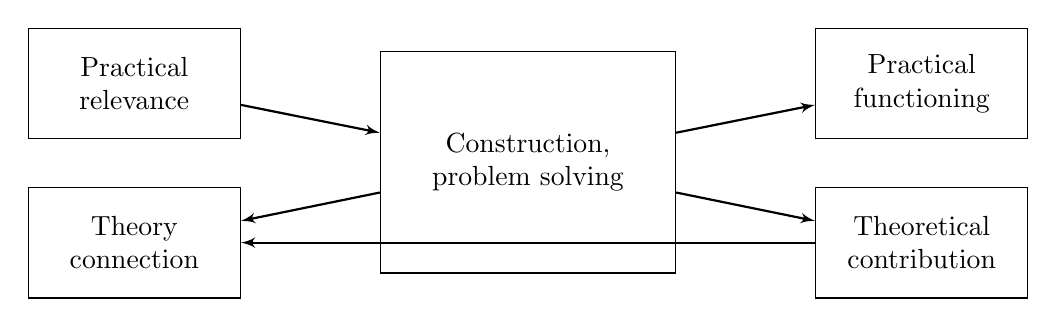
\begin{tikzpicture}[
    start chain=going below,    % General flow is top-to-bottom
    node distance=6mm and 50mm, % Global setup of box spacing
    ]
% ------------------------------------------------- 
\tikzset{
  base/.style={draw, on chain, on grid, align=center, minimum height=4ex},
  proc/.style={base, rectangle, minimum height=4em, text width=7em},
  big/.style={base, rectangle, minimum height=8em, text width=10em},
   line/.style={draw, thick, -latex'}
}
% -------------------------------------------------
% Placing the nodes

\node [proc] (rel) {Practical relevance};
\node [proc] (con) {Theory connection};
\node [big, right=of rel, yshift=-1cm] (prb) {Construction, problem solving};
\node [proc, right=of prb, yshift=1cm] (fun) {Practical functioning};
\node [proc] (ctr) {Theoretical contribution};

\path [line] (rel) -- (prb);
\path [line] (prb) -- (fun);
\path [line] (prb) -- (ctr);
\path [line] (prb) -- (con);
\path [line] (ctr) -- (con);

\end{tikzpicture}
\caption{Constructive research model adapted from \citet{kasanen1993constructive}} \label{fig:constructive}
\end{figure}

Reasoning follows an abductive logic path where an initial observation in the "real" world is brought under theoretical scrutiny and modeling. The subsequent rationalisation is the then returned to inductive empirical appraisal and generalized back into theory and a new refined model. \citep{josephson1996abductive}

% todo: add description of interview process and picture or research structure

\section{Study organisation and thesis structure}
\label{section:structure}
% TODO add num of parts
This master's thesis study is divided to x parts. First, necessary background information on software integration testing, Wärtsilä's systems architecture, and information systems is presented in Chapter \ref{chapter:background}. The chapter also includes a requirements analysis based on interviews conducted at the company. Next, integration testing frameworks are explored by looking at existing models and a synthesis on their strategical, tactical, and operational nature is given. Along with a more generic look at integration testing theory, Chapter \ref{chapter:frameworkanalysis} breaks down the framework into process components, which are then put together in Chapter \ref{chapter:frameworkproposal} into a new framework model tailored for Wärtsilä.

% testing automation are examined. efficient defect management. 
The empirical part of the study evaluates a working prototype of the new testing framework. It presents a proof-of-concept implementation and reflects on the solution in respect to previous academic research and applicability in solving Wärtsilä's underlying business problems. The last chapter also contains critical appraisal of both the theoretical and empirical part of the study and if the thesis met its objectives.

% todo rephrase
The story arc of the thesis is not unlike putting together Lego. In the background chapter the constructor can peruse the contextual setting and rough guidelines for assembly, while in the next part, he/she is shown ready models, built by experts, for reference and inspiration. After this, the box is merrily torn open and the bricks scattered on the floor. The builder can pore over individual pieces and see how they they appear, feel, and stick together. A prototype construct is made and compared to expectations and presented to interested parties.

\chapter{Research background}
\label{chapter:background}

% defining process, financal gain tied to company objectives
% what should be measured? add to workshop agenda?
% rquirements analysis should be done well so as to avoind further issues or issues in commuication
% process must be defined first, then the actual IT system
% 1. haasteet 2. käyttäjät 3. käyttötapaukset 4. tietosisältöjen määrittely

To help fully grasp the key questions in the thesis, the reader is furnished with necessary background information about software (integration) testing, its merits, and the testing need at Wärtsilä. The theoretical and practical insights serve as reference when constructing the testing framework. 

The first two chapters examine software testing from a more general perspective. The method of research is literature study. The latter two chapters investigate Wärtsilä's context of need and enumerates requirements for the framework, which are based on an interview with a testing expert at Wärtsilä.

\section{Testing software systems}

Testing is an essential part of software engineering. Without a degree of confidence of sound operation and functional integrity, systems accumulate great risk and may ultimately produce more harm than benefit. Controlled testing reduces the number of incidents that would otherwise be discovered in the live environment and fixing which would be very expensive. \citep{jenkins2008software, liu2009unified} In a similar fashion, testing can point to ways the systems can be improved. For example, a system that is fluid and easy to use does not incur as many service and maintenance or information requests. And lastly, testing helps decision makers understand the risks involved in IT applications and services.

Along with the functionality of the system, tests should also be applied to non-functional aspects such as performance and usability, because these also determine the validity of the system under test (SUT). Verifying that specified functions are implemented is not enough, but the system must reach and perform at an adequate level of service. % todo lähde

Traditionally, testing is grouped to unit, integration, and system levels \citep{jenkins2008software, burnstein2003practical}. Unit testing is assuring that individual software modules and functions perform to specifications. When these are paired or grouped, the resulting connections and integrations must also be tested. Finally, system testing refers to proofing the finished software suite with a suitable array of use cases. 

%todo reference for first sentence?
The distinction between unit, integration, and system tests is not clear, however. Some authors consider end-to-end integration testing akin to system tests. \citet{duvall2007continuous} writes about \emph{component testing} synonymous with integration testing. \citet{pezze2008software} and \citet{benz2007combining} consider this an intermediary stage between unit and integration/system tests while \citet{burnstein2003practical} likens component testing to unit testing. IEEE defines integration testing as testing in which \emph{"software components, hardware components, or both are combined and tested to evaluate the interaction among them"} \citep{ieee2010systems}.

% What to test
The fluid progression from atomic unit tests to holistic system tests strongly reflects the software development process. Naturally, software has to be tested to during and after initial development, but there are other reasons, too. Any change in code or specifications, the environment, or testing policy, or plans can act as a trigger for testing. Systematically repeating a set of tests to ascertain changes (like fixes) have not introduced new errors to previously functional code is called regression testing. The execution of regression tests is typically automated (TODO references). A nearby concept, \textit{retesting} refers to examining if a fix has actually resolved a software bug \citep{jenkins2008software}.

Continuous integration (CI) is a further approach where testing is done frequently as changes are made to source code. The purpose is to weed out issues and defects related to component interoperation before they take root can cause major trouble. \citet{duvall2007continuous} described continuous integration as:

\begin{adjustwidth}{2.5em}{0pt}
\small
\emph{"A software development practice where members of a team integrate their work frequently, usually each person integrates at least daily --- leading to multiple integrations per day. Each integration is verified by an automated build (including test) to detect integration errors as quickly as possible. Many teams find that this approach leads to significantly reduced integration problems and allows a team to develop cohesive software more rapidly."}
\normal
\end{adjustwidth}

% move integration testing stuff here?

\section{Why automated testing?}

% Write about what processes are already defined and argue that there is no overlap. What to do. technique how to do. Does not assume overall test steering responsibilities, the two are separated and not dependent so they can be updated individually.

The bigger and the more numerous information systems are, the more problems are likely to arise. Software failures may result in squandered time and money, and even loss of life \citep{leveson1993investigation, defense1992software}. The growing pressures for delivering quality and controlling IT risks are reflected on software testing. This in turn creates a demand for testing automation. Already in 1976 \citet{myers1976software} stated that maintenance and testing account for 75\% of software costs.

The oft-cited reasons for testing automation are improving software quality and cost-efficiency: harnessing the power of computers helps expedite the testing process as well as reduce the amount of manual work. \citet{fewster1999software} give a more complete list of automation benefits:

\begin{itemize}
\item Reusing tests on a new version of the system
\item Reusing tests in a new project
\item Running tests more often
\item Performing tests which would be difficult or impossible to do manually (e.g. performance tests)
\item Freeing test engineers to do more rewarding work
\item Consistency and repeatability of tests
\item Increased confidence due to increased and systematic testing
\item Shortening development time, faster time to market
\end{itemize}

Naturally, automation comes with its downsides and risks, some of which are not insignificant. These will be explored later in Section \ref{section:pitfalls}.

\section{Testing at Wärtsilä}

Wärtsilä is a Finnish technology company providing lifecycle power solutions for the marine and energy markets. The three main business units marine solutions produces engines primarily for cruise ships, power plants designs and constructs plants, and services offer a range of maintenance services and support to Wärtsilä's customers. \citep{wartsila2013web}

% add mention of interview

Integration testing is particularly important at Wärtsilä because the company typically outsources IT development. This pushes unit testing responsibilities to the supplier, while solution integration remains Wärtsilä's concern and responsibility. A flexible and well-defined integration testing process framework can serve many development projects to come. To date, there have been cases with unnecessary duplicate work. In a recent ERP update effort the scale of and need for testing became evident to Wärtsilä. A framework guiding the testing process and automating a part of it could significantly reduce costs and risks as well as project execution time.

% references to these? what can be included?
Wärtsilä's business rests on over 50 different systems, for example enterprise and customer resource planning, product data management, warehouse control, and financial systems, which are intersected by information exchange processes. The system architecture is built on the service-orientation principle (SOA), where individual systems or software components lend their services to be called by other systems' services through a shared channel, the enterprise service bus (ESB). Adapters and application programming interfaces (APIs) provide a means to access and use systems irrespective of their internal composition (e.g. programming language). This permits adding new services and replacing or removing old ones incrementally, but does not remove the challenges related to testing. A change in even one of the systems can potentially break one or more process chains. 

% remove picture?
\begin{figure}
\centering
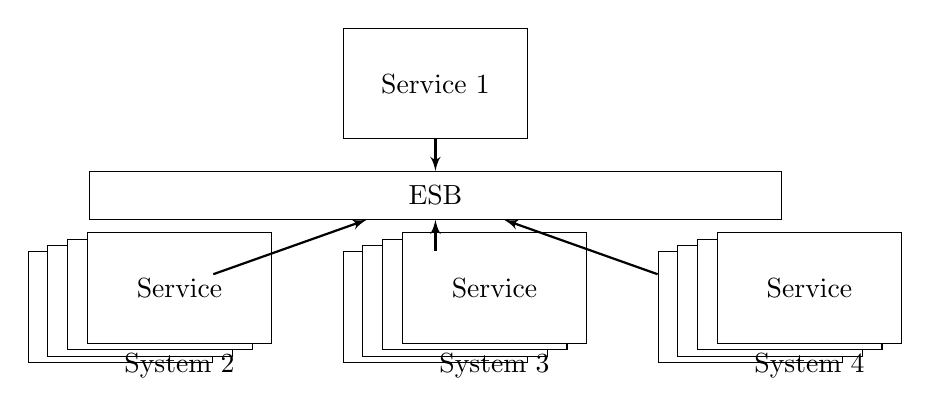
\begin{tikzpicture} [
   start chain=going below,        % General flow is top-to-bottom
    node distance=4mm and 40mm,    % Global setup of box spacing
    ]
% ------------------------------------------------- 
\tikzset{
  base/.style={draw, on chain, on grid, align=center, minimum height=4ex},
  rect/.style={base, rectangle, minimum height=4em, text width=6em},
  bus/.style={base, rectangle, minimum width=25em, text width=8em},
  line/.style={draw, thick, -latex'},
}
    \node [rect, xshift=1.25cm] (s1) {Service 1};
    \node [bus] (esb) {ESB};
  
    \node [rect, xshift=-4.00cm] (s21) {};
    \node [rect, xshift=0.25cm, yshift=1.90cm, fill=white] (s22) {};
    \node [rect, xshift=0.25cm, yshift=1.90cm, fill=white] (s23) {};
    \node [rect, xshift=0.25cm, yshift=1.90cm, fill=white, label=below:{System 2}] (s24) {Service};
    
    \node [rect, right=of s21] (s31) {};
    \node [rect, xshift=0.25cm, yshift=1.90cm, fill=white] (s32) {};
    \node [rect, xshift=0.25cm, yshift=1.90cm, fill=white] (s33) {};
    \node [rect, xshift=0.25cm, yshift=1.90cm, fill=white, label=below:{System 3}] (s34) {Service};
    
    \node [rect, right=of s31] (s41) {};
    \node [rect, xshift=0.25cm, yshift=1.90cm, fill=white] (s42) {};
    \node [rect, xshift=0.25cm, yshift=1.90cm, fill=white] (s43) {};
    \node [rect, xshift=0.25cm, yshift=1.90cm, fill=white, label=below:{System 4}] (s44) {Service};
  
    \path [line] (s1) -- (esb);
    \path [line] (s21) -- (esb);
    \path [line] (s31) -- (esb);
    \path [line] (s41) -- (esb);
    
\end{tikzpicture}
\caption{Service-oriented architecture} \label{fig:soa}
\end{figure}

% add reference
Since the systems undergo continuous changes, like improvements, upgrades, fixes, pilots, etc., the need for regression tests is common. Ideally, a prepared test set could be executed by issuing a simple command \citep{duvall2007continuous}. In addition to the benefits listed earlier, testing, if executed continuously, would also provide an up-to-date view on the status of systems. This improves quality and transparency of information and can thereby be argued to aid decision-making.

In an interview with a testing expert at Wärtsilä, it was revealed that current testing at Wärtsilä is ad-hoc. There is no universal testing framework. A set of tools, which include for instance a bug tracker tool and a UI scripting tool, have been adopted and are used on a mix-and-match basis. There is also a monitoring tool in which failed communication is flagged and which can roughly indicate the existence of bugs. Organization test strategy, policy, and testing processes are described and defined, but the practical testing approach is set by project managers or project test managers.

Requirements and specifications are collected among solution key users and managers. Unit tests are performed by the vendor, which is followed by integration tests in Wärtsilä's test environment executed by Wärtsilä's technical experts and possibly aided by the vendor. Next, system tests are done by the solution manager, who then passes the solution forward to business key users for verification testing. % has verification testing been introduced  

Test cases are constructed manually and are not maintained. After a development project is closed and moves to \eph{live maintenence mode}, new cases are created when needed as new features or enhancements are released. In some few cases, a battery of regression tests is maintained. Testing results and found incidents are logged to a bug tracking system, or collected in shared files or email conversations. 

The reuse and reusability of testing objects is minimal. Steps have been taken to standardize the testing process, to identify the most important points of improvement, and raise the maturity level of testing to gradually establish the preconditions for an automated and controlled organisation-wide process. Introducing the new integration testing framework is a grand undertaking requiring the participation of many stakeholders. A complex, inflexible or overly prescribing model will probably not find much use.

% a jumble systems plugged into the common esb, critical system, managing risk, 
% rest regime is a framework

\section{Requirements for the integration testing framework}  

Three technical experts at Wärtsilä shared their views on the framework early on in interviews conducted by the researcher. The interviews, approximately an hour in length, were loosely structured and had no presumptions about the nature of the framework-to-be. The mission was to elicit Wärtsilä's requirements for integration testing including technical, functional, and practical aspects. The two latter interviewees were, however, presented with findings from earlier interviews for their opinion and the addition of any further comments or clarifications.

The first interviewee, who also commissioned the work, acts as technical integrations architecture expert. Confirmed in the interview, the core test cases or integration message exchanges are of synchronous or asynchronous type. 

In the former, a client application sends a request, which passes through the integration service and transformations along to the ESB from where it continues on to the receiving system. This immediately returns a reply which travels the same route in the opposite direction. Consequently, the framework needs a tool capable of sending and receiving these messages and presenting the final results to the tester for examination.

The more tricky asynchronous messaging method, where no message is returned (at least not immediately), makes verification more difficult. Visibility to the end system is required. Since end system functionality is not in the test scope, intercepting the message after it has been subjected to integration transformations but before it reaches its final destination, and ascertaining it is correct by comparing it to an example, would suffice. Mocking services and systems or redirecting messages are practical ways to achieve this.

The integrations expert also pointed to the possibility of recording messages in the current production environment so that they might be used as input data in test cases, and as reference when ascertaining the integration-transformed messages are of correct form. 

Finally, a list of messaging protocols that should be supported by the framework was made.

The second interviewee, responsible for enterprise architecture and governance, concurred with the previous requirements and added three scenarios where integration testing is needed. Firstly, integration regression testing in a testing environment is needed when systems are updated and before changes are deployed into the production environment. Second, IT projects require end-to-end integration verification tests throughout the course of the project to be performed in the development or quality assurance environment. Finally, an integration health check or smoke test in production should be enabled to quickly flag any errors and direct to problem areas. 

The third interviewee, an solutions architect, advocated using existing resources, such as manual test scripts, in implementing integration testing and the method of creating test cases should be well documented so as to help future testers adhere to and use the framework's testing process. Now specific method for test creation was endorsed, however.

All of the collected requirements are shown in Table \ref{fig:reqstable}.
%Tommi

\begin{figure}[H]
\begin{center}
\rowcolors{1}{lightgray}{white}
\renewcommand{\arraystretch}{2}
\begin{tabular}{ l p{10cm} }
  \hline                        
  R1 & It shall be possible to run test cases. \\ 
  R2 & It shall be possible to schedule automatic test runs. \\ 
  R3 & It shall be possible to write and generate test cases. \\ 
  R4 & It shall be possible to capture and replay messages. \\
  R5 & It shall be possible to generate mock services or stubs. \\
  R6 & It shall be possible to validate test results automatically. \\
  R7 & HTTP/XML, JDBC, and (S)FTP messaging protocols shall be supported. \\
  R8 & It shall be possible to generate test loads, and conduct load tests. \\
  R9 & It shall be possible to generate test loads and conduct stress tests. \\
  R10 & It shall be possible to monitor test results and performance metrics. \\
  \hline  
\end{tabular}
\end{center}
\caption{Requirement table}} \label{fig:reqstable}
\end{figure}

The requirements collected is an excellent yardstick when selecting framework technologies or tools, and in evaluation different testing models and approaches. It also points to interesting areas of integration testing theory, such as test case and service mock-up creation.

\section{Summary}

This chapter reviewed the theoretical premises of integration testing and the practical context of the to-be framework at Wärtsilä. Integration testing can be done pairwise moving systematically over the entire system or through more system test oriented end-to-end tests where multiple integrations are tested in one test scenario. Previous research has proved that controlled early testing reduces development and maintenance costs and is required throughout the software life-cycle. % Todo lähde 

Wärtsilä's relatively conventional technological and business environments should allow for --- and benefit from --- testing automation, which makes the thesis highly relevant. The case specific requirements collected and presented in the chapter serve as basis for evaluating testing solutions and building the framework.

\chapter{Looking for a testing framework}
\label{chapter:frameworktheory}

This chapter explores the theoretical base for a framework. First it examines integration and testing strategies in respect to frameworks and presents approaches to integration testing developed earlier. The thesis postulates that testing strategy and framework selection are inseparable in that strategy determines the general testing approach, but the technical limitations of frameworks impose restrictions on strategic decisions, too. A suitable fit must exists between IT strategy and information system infrastructure and processes \citep{henderson1993strategic}. To a reasonable degree, a framework should be flexible enough to adapt to individual project needs.

% no single test auomation solution M. Fewster and D. Graham. Software Test Automation. Addison-Wesley, 1999.

From an IT or software perspective, a framework is understood as an abstract technology or library intended for a purpose \citep{johnson1988designing}. In the scope of this thesis, the framework concept is extended to the overall process workflow related to (integration) testing. While a technology may be a part of the framework, the framework itself is technology-agnostic and only sets requirements for functionality. \citet{pezze2008software} considers it an application skeleton, \textit{"a circuit board with empty slots for components"}. 

\citet{fewster1999software}, \citet{liu2009unified}, \citet{huang2008surrogate}, and \citet{laukkanen2006data} present frameworks that span the integration testing process start to end and which are presented in this chapter. These are presented in Figures \ref{fig:autotestprocess}, \ref{fig:liu}, \ref{fig:huang}, and \ref{fig:laukkanen}. The models show that frameworks combine different tools for different process steps along the workflow chain.

\section{Integration test automation model}

\citet{fewster1999software} present an integration testing automation process, based on a test harness tool called Autotest, which author Mark Fewster worked on during his employment at Racal-Redac. The straightforward model in Figure \ref{fig:autotestprocess} shows a process extending from input and instructions to actual testing, then to output and expected output comparison and culminates in a test report.

\begin{figure}[H]
\centering
% =================================================
\pgfdeclarelayer{marx}
\pgfsetlayers{main,marx}
% -------------------------------------------------
% Start the picture
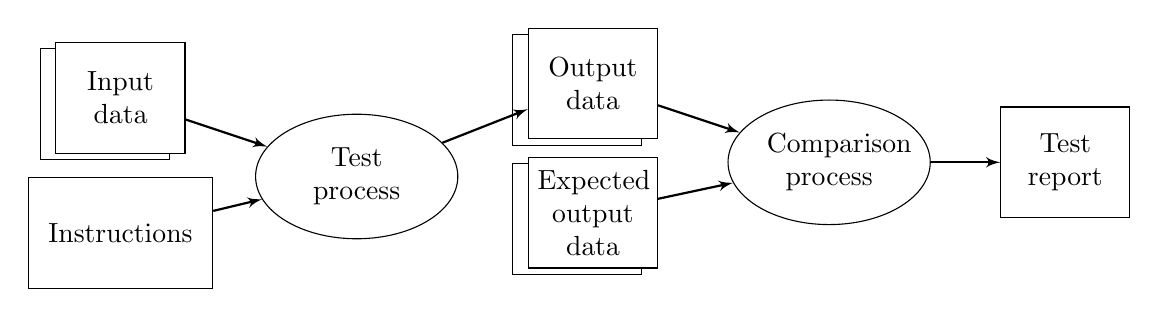
\begin{tikzpicture}[
    start chain=going below,    % General flow is top-to-bottom
    node distance=3mm and 30mm, % Global setup of box spacing
    ]
% ------------------------------------------------- 
\tikzset{
  base/.style={draw, on chain, on grid, align=center, minimum height=4ex},
  proc/.style={base, rectangle, minimum height=4em, text width=4em},
  proclong/.style={base, rectangle, minimum height=4em, minimum width=6em, text width=6em},
  elli/.style={base, ellipse, minimum height=4.5em, text width=4.5em},
  line/.style={draw, thick, -latex'}
}

\node [proc] (datain0) {};
\node [proc, fill=white, yshift=1.80cm, xshift=0.20cm] (datain) {Input data};
\node [proclong] (ins) {Instructions};

\node [elli, right=of datain, yshift=-1.00cm] (prc) {Test process};

\node [proc, right=of prc, xshift=-0.20cm, yshift=1.10cm] (dataout0) {};
\node [proc, yshift=1.80cm, xshift=0.20cm, fill=white] (dataout) {Output data};

\node [proc, xshift=-0.20cm] (exp0) {};
\node [proc, fill=white, yshift=1.80cm, xshift=0.20cm,] (exp) {Expected output data};

\node [elli, right=of dataout, yshift=-1.00cm] (com) {Comparison process};
\node [proc, right=of com] (rep) {Test report};

\path [line] (datain) -- (prc);
\path [line] (ins) -- (prc);
\path [line] (prc) -- (dataout);
\path [line] (dataout) -- (com);
\path [line] (exp) -- (com);
\path [line] (com) -- (rep);

\end{tikzpicture}
\caption{Automated integration test process adapted from \citep{fewster1999software}} \label{fig:autotestprocess}
\end{figure}

Each test is defined by the input data and instructions at the upper reaches of the process chain. The data should be complete enough for computational test execution. Comparisons are made with an array of different tools depending on the file format, though format support has come some way since Fewster's experiment.

The framework requires manual setup, for instance manual validation and storing of the expected outcome must be done before any tests can be automatically run. After some initial work, Fewster was able to squeeze out a 7 person-week reduction compared to manual testing \citep{fewster1999software}.

\section{Surrogate system}

\citeauthor{huang2008surrogate}'s \citeyearpar{huang2008surrogate} model, a precursor to the authors unified testing framework presented in figure \ref{fig:liu}, is concerned with the testing environment arrangements related to surrogates or mock services, but figure \ref{fig:huang} already shows a clear framework structure stretching from test case generation to verification of system functionality. The area around simulating components is the area of focus, though both of the authors' models attempt to elaborate on the subprocesses and tasks that lie upstream on the testing process chain. \citep{huang2008surrogate}

\begin{comment}
\begin{figure}[H]
\centering
% =================================================
\pgfdeclarelayer{marx}
\pgfsetlayers{main,marx}
% -------------------------------------------------
% Start the picture
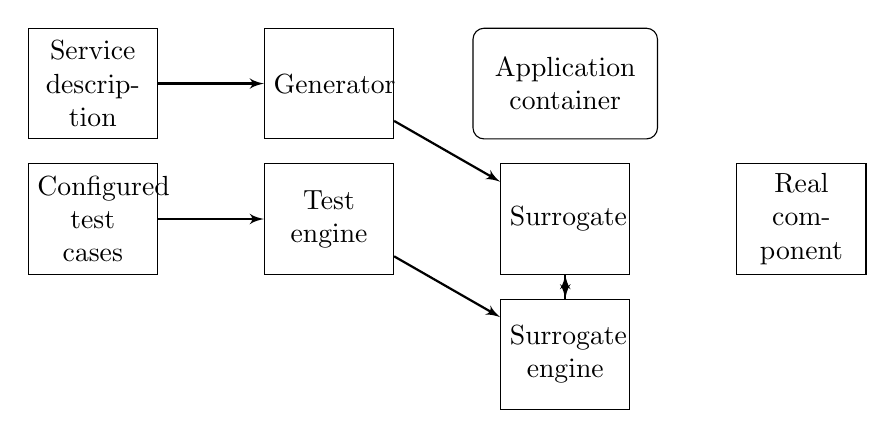
\begin{tikzpicture}[
    start chain=going below,    % General flow is top-to-bottom
    node distance=3mm and 30mm, % Global setup of box spacing
    ]
% ------------------------------------------------- 
\tikzset{
  base/.style={draw, on chain, on grid, align=center, minimum height=4ex},
  proc/.style={base, rectangle, minimum height=4em, text width=4em},
  cont/.style={base, rectangle, rounded corners, minimum height=4em, minimum width=6em, text width=6em},
  elli/.style={base, ellipse, minimum height=4.5em, text width=4.5em},
  line/.style={draw, thick, -latex'}
}
\node [proc] (desc) {Service description};
\node [proc] (tcs) {Configured test cases};
\node [proc, right=of desc] (gen) {Generator};
\node [proc] (ten) {Test engine};
\node [cont, right=of gen] (app) {Application container};
\node [proc] (sgt) {Surrogate};
\node [proc] (sen) {Surrogate engine};
\node [proc, right=of sgt] (rea) {Real component};
\path [line] (desc) -- (gen);
\path [line] (gen) -- (sgt);
\path [line] (tcs) -- (ten);
\path [line] (ten) -- (sen);
\path [line] (sgt) -- (sen);
\path [line] (sen) -- (sgt);
\end{tikzpicture}
\caption{Surrogate system architecture \citep{huang2008surrogate}} \label{fig:surrogate}
\end{figure}
\begin{comment}

\begin{figure}[H]
  \begin{center}
    \includegraphics[width=13cm]{huang_et_al_framework.png}
    \caption{Surrogate system architecture \citep{huang2008surrogate}}
    \label{fig:huang}
  \end{center}
\end{figure}

% The surrogate engine provides two kinds of technology independent interfaces: interface to configure component behavior and interface to get simulated behavior.

\begin{comment}
\begin{figure}[H]
  \begin{center}
    \includegraphics[width=13cm]{huang_testing_process.png}
    \caption{The testing processes by \citet{huang2008surrogate}}
    \label{fig:huangtesting} 
  \end{center}
\end{figure}
\end{comment}

In the surrogate system, the environment is made of the application container which may or may not contain parts or the whole of the system under test and in which surrogates, or mock services or stubs, are deployed. Again, the many interfaces in the framework are highlighted. The surrogate generator has a component for configuring surrogates as well as a library of functions for imitated behaviour.

\citet{huang2008surrogate} instruct that before test execution the necessary surrogates should be defined by test case and deployed. Before test case execution, the surrogate component availability is checked. To achieve true automation, then, such environmental setup should also be automated.

% data driven testing another way of saying automated testing?

\section{A unified testing framework}

The \citet{liu2009unified} model (Figure \ref{fig:liu}) includes processes, objects, and agents. Based on a UML sequence diagrams, the test generator semi-automatically creates test cases later submitted to the execution engine. Test runs are facilitated by a surrogate engine or engines which mock external systems. After execution, IBM's proprietary ITCAM technology aggregates execution traces together with the help of a trace correlator, which then pass the traces for transformation into a standard format. The test cycle is finished off by verification on the integration test case and execution trace and returning the result to the execution engine.

The surrogate \emph{generator} was conspicuously left out of the model. The authors chose to scope out this part of the framework and focus on the testing execution process rather than preconfiguration.

The researchers separated test case structure and logic for platform independence. The test logic and configuration settings were encoded in separate XML files. The unified testing framework was built to be technology independent so 
separate plug-ins were created for the SOA context and technologies.

\begin{figure}[H]
  \begin{center}
    \includegraphics[width=13cm]{liu_et_al_framework.png}
    \caption{Unified testing framework \citep{liu2009unified}}
    \label{fig:liu}
  \end{center}
\end{figure}

The unified testing framework was tried out in relatively small-scale experiments, but successfully uncovered bugs early in development supporting the authors' claims. The framework also helped find different kinds of bugs and didn't appear to have a bias towards uncovering a certain kind of defect \citep{liu2009unified}.

\section{Data-driven testing framework}

In \citeauthor{laukkanen2006data}'s \citeyearpar{laukkanen2006data} data and keyword driven testing model (figure \ref{fig:laukkanen}) testing is divided into modules for \emph{test design}, \emph{test execution}, and \emph{test monitoring}. A data-driven model, automation is enabled by correctly formatted and stored test inputs, test data, and driver scripts.

A test design system is used to create and edit tests cases. In practice, the system could simply be a spreadsheet or HTML editor. According to \citet{laukkanen2006data} the test monitoring system is used for controlling test execution and checking test results. The visualized results are in the form of low-level text logs or more visually-pleasing HTML.

At the heart of the framework lies the test execution system which houses test libraries, driver scripts, and the test data parsers, as well as the logger and report generator utilities. The monitoring system fires driver scripts which use functions in the test libraries and modules to perform test actions. The parser manages test data and converts to the right format. The logger collects relevant execution information which is also used as input in test reports. Both logs and reports can be viewed in the monitoring system. \citep{laukkanen2006data}

\begin{figure}[H]
  \begin{center}
    \includegraphics[width=13cm]{laukkanen_framework.png}
    \caption{Laukkanen's testing framework \citep{laukkanen2006data}}
    \label{fig:laukkanen} 
  \end{center}
\end{figure}

Where the two first models essentially depict a loop and treat continuous testing as implicit, the keyword-driven model instead offers a monitoring step which overlays verification processes where a view to system status and health is more clearly separated from the testing execution. Naturally, a batch of test cases can be set to run to update the status. \citeauthor{laukkanen2006data}'s \citeyearpar{laukkanen2006data} model also supports the notion that a full framework should contain tools for the key processes test case generation, test execution, and verification (or monitoring).

\citet{laukkanen2006data} piloted the data and keyword driven framework in Windows application testing.

\section{Models summary}

The testing frameworks or models introduced in this chapter have striking similarities and subtle individual connotations. All models save for \citeauthor{huang2008surrogate}'s \citeyearpar{huang2008surrogate} surrogate architecture really only a part of the whole continuous integration process they later touch on, can be argued to follow a three step process of \emph{generating necessary input} (cases, surrogates, test data), \emph{running the test scripts}, and finally \emph{verifying and comparing results}. The process funnels are comparable to e.g. \citeauthor{davenport1993process}'s \citeyearpar{davenport1993process} definition of a business process taking an input and producing a result or indeed a software method that takes some parameters and return some output.

% Alternatively: So as not to get too distracted by the rather pragmatic and techincal models, a more holistic...
Since all of the models are rather pragmatic and technical, a more holistic perspective is reserved for further analysis of the nature of the integration testing framework. Figure \ref{fig:funnel} presents a framework on three levels of abstraction (horizontal dimension) and the process dimension (vertical) just discussed.
%Pace of integration, rate of automation, definition for I/O process

\begin{figure}[H]
\centering
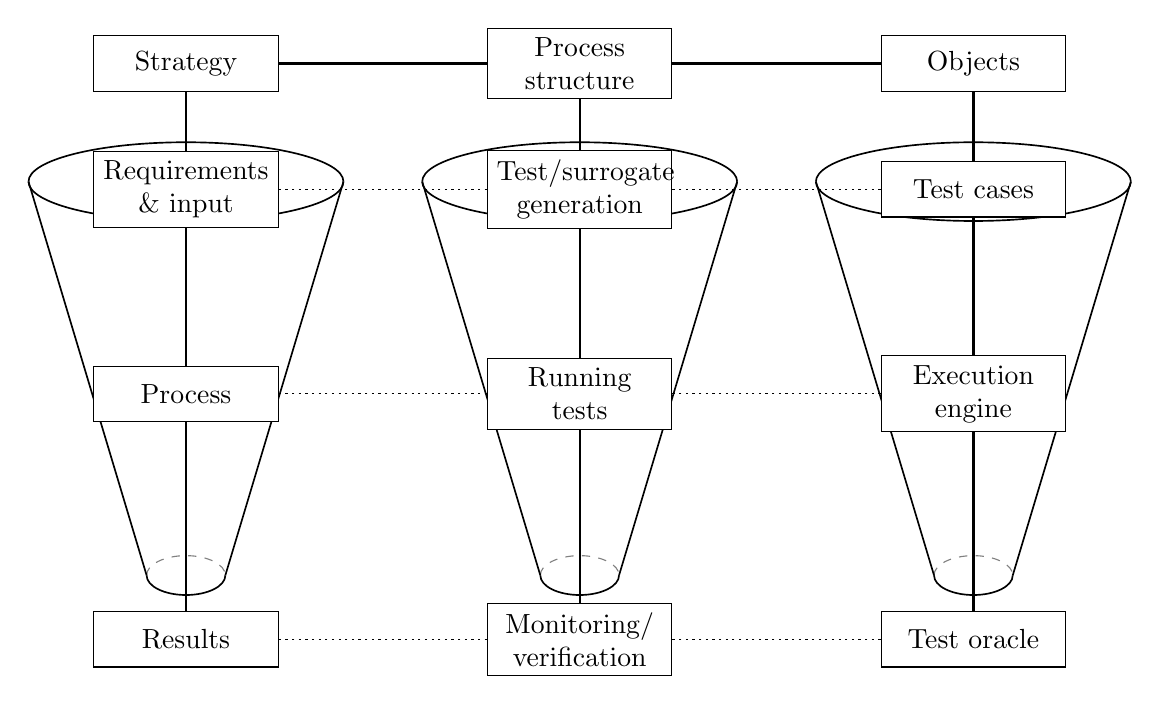
\begin{tikzpicture} [ 
   start chain=going below,         % General flow is top-to-bottom
    node distance=10mm and 50mm,    % Global setup of box spacing
    ]
% ------------------------------------------------- 
\tikzset{
  base/.style={draw, on chain, on grid, align=center, minimum height=4ex},
  rect/.style={base, rectangle, minimum height=2em, text width=6em},
  line/.style={draw, thick}, %, -latex'},
  dots/.style={draw, dotted} %, -latex'}
}

    \draw[semithick] (-5,0) arc (180:0:2 and 0.5);                  % cone 1: top ellipse top arc
    \draw[dashed,color=gray] (-3.5,-5) arc (180:0:0.5 and 0.25);    % cone 1: bottom ellipse top arc
    \draw[semithick] (-3.5,-5) arc (-180:0:0.5 and 0.25);           % cone 1: bottom ellipse bottom arc
    \draw[semithick] (-5,0) arc (-180:0:2 and 0.5);                 % cone 1: top ellipse bottom arc
    \draw[semithick] (-5,0) -- (-3.50,-5);                          % cone 1: left side
    \draw[semithick] (-1,0) -- (-2.50,-5);                          % cone 1: right side
    
    \draw[semithick] (0,0) arc (180:0:2 and 0.5);                   % cone 2: top ellipse top arc
    \draw[dashed, color=gray] (1.5,-5) arc (180:0:0.5 and 0.25);    % cone 2: bottom ellipse top arc
    \draw[semithick] (1.5,-5) arc (-180:0:0.5 and 0.25);            % cone 2: bottom ellipse bottom arc
    \draw[semithick] (0,0) arc (-180:0:2 and 0.5);                  % cone 2: top ellipse bottom arc
    \draw[semithick] (0,0) -- (1.5,-5);                             % cone 2: left side
    \draw[semithick] (4,0) -- (2.5,-5);                             % cone 2: right side

    \draw[semithick] (5,0) arc (180:0:2 and 0.5);                   % cone 3: top ellipse top arc
    \draw[dashed, color=gray] (6.5,-5) arc (180:0:0.5 and 0.25);    % cone 3: bottom ellipse top arc
    \draw[semithick] (6.5,-5) arc (-180:0:0.5 and 0.25);            % cone 3: bottom ellipse bottom arc
    \draw[semithick] (5,0) arc (-180:0:2 and 0.5);                  % cone 3: top ellipse bottom arc
    \draw[semithick] (5,0) -- (6.5,-5);                             % cone 3: left side
    \draw[semithick] (9,0) -- (7.5,-5);                             % cone 3: right side

    \node [rect, xshift=-3.0cm, yshift=1.5cm, fill=white] (stg) {Strategy};
    \node [rect, yshift=0.25cm, fill=white] (req) {Requirements \& input};
    \node [rect, yshift=-0.75cm, fill=white] (prc) {Process};
    \node [rect, yshift=-1.4cm, fill=white] (rlt) {Results};
    
    \node [rect, right=of stg, fill=white] (fmw) {Process structure};
    \node [rect, right=of req, fill=white] (tcg) {Test/surrogate generation};
    \node [rect, right=of prc, fill=white] (run) {Running tests};
    \node [rect, right=of rlt, fill=white] (mon) {Monitoring/ verification};
    
    \node [rect, right=of fmw, fill=white] (art) {Objects};
    \node [rect, right=of tcg, fill=white] (tcs) {Test cases};
    \node [rect, right=of run, fill=white] (exe) {Execution engine};
    \node [rect, right=of mon, fill=white] (out) {Test oracle};
    
   % \node [rect, below=of mon, yshift=-1.0cm, fill=white] (pit) {Pitfalls};
     
    \path [line] (stg) -- (fmw);
    \path [line] (fmw) -- (stg);
    \path [line] (fmw) -- (art);
    \path [line] (art) -- (fmw);
    
    \path [line] (stg) -- (req);
    \path [line] (req) -- (prc);
    \path [line] (prc) -- (rlt);
    
    \path [line] (art) -- (tcs);
    \path [line] (tcs) -- (exe);
    \path [line] (exe) -- (out);
    
    \path [line] (fmw) -- (tcg);
    \path [line] (tcg) -- (run);
    \path [line] (run) -- (mon);
    
    \path [dots] (run) -- (prc);
    \path [dots] (prc) -- (run);
    \path [dots] (run) -- (exe);
    \path [dots] (exe) -- (run);
    
    \path [dots] (req) -- (tcg);
    \path [dots] (tcg) -- (req);
    \path [dots] (tcg) -- (tcs);
    \path [dots] (tcs) -- (tcg);
    
    \path [dots] (rlt) -- (mon);
    \path [dots] (mon) -- (rlt);
    \path [dots] (mon) -- (out);
    \path [dots] (out) -- (mon);
 
\end{tikzpicture}
\caption{Process levels in integration testing} \label{fig:funnel}
\end{figure}
%remove arrows?

The framework is analyzed from a strategic, technical/structural, and component level. Starting from the left, general testing strategy and requirements are accepted as premises and translated into a framework structure, largely uniform, but flexible enough to conform to minor project idiosyncrasies. In each separate case framework scope is outlined by specifications and agreements e.g. on security policy or service level, and more formally described in a test plan, which typically includes test objectives, responsibilities and schedules, a list of necessary tools, process descriptions, and success criteria \citep{myers1976software}.

The structure should be robust or modular enough to be separable into clear and concrete constituent parts, like test cases, in human or machine readable form. These should be constructed with regard the framework strategy and structure scope. The modularity permits the fluent addition of new test cases, integrations, or other components to the framework.

\begin{comment}
The testing process can vary in its mode of execution or degree of automation. In what is perhaps the most extreme case, test case are run automatically every time a change is committed to system source code. This approach is called continuous integration (CI). 
\end{comment}

% test harness ephasizes stubs and mock-ups

\chapter{Deconstructing the integration testing framework}
\label{chapter:frameworkanalysis}

% drop something in funnel runs automatically 
This chapter examines individual components and subprocesses of integration testing, based on the models and model synthesis derived in the previous chapter. The first section enumerates important testing strategy decisions, while the next concentrates on practical questions and what options and tools there are to implement the strategy. The final section evaluates the framework for a component and maintenance perspective.

% testing strategy
\section{Testing strategy}

Testing strategy is broken down to aspects of coverage-efficiency requirements, process design, and how test results are used to drive quality and further improve testing practices. Precisely, the first strategy choice is test case selection and design, the second the test control and management model, and the last test and framework improvement through feedback. % does this need a reference

\subsection{Requirements for coverage and efficiency}

One can observe that because testing must only provide reasonable confidence in system performance, it can be selective. Not everything should or indeed can be tested. Focusing on a part of the whole system saves time and costs. It is however essential to model and understand the system flow and which part of it should be tested. If only a part of system is known to have changed, testing can be limited to the new functionality \citep{bhuyan2012survey}. 

Similarly, effort put to test case production should be defined by planning coverage and case selection. Ideally, the set of cases provides minimum required coverage based on testing strategy and business strategy criteria. 

Overall test effectiveness can be measured by how many cases were executed out of the set of necessary cases and feature testability by how many test cases are necessary for satisfying a criterion \citep{linnenkugel1990test}. Therefore attention must be spent on both selecting the method of execution and test criteria. 

The most common way to evaluate coverage is based on control flow, which simply means the order in which individual statements, instructions or function calls occur. Visualizing the program process flows can help understand the program logic, potential features to test, and guide the construction of test cases, too. \citep{burnstein2003practical} 

\citet{linnenkugel1990test} present a flow-oriented coverage hierarchy of node, relation, call, sequence, and loop coverage measures. For integration testing, individual components (modules) are nodes and integrations are relations (call statements). \citeauthor{linnenkugel1990test}'s \citeyearpar{linnenkugel1990test} coverage criteria include:
\begin{itemize}
\item \emph{all-modules} requires that every module is executed at least once 
\item \emph{all-relations} requires that the calling relation between modules is executed at least once
\item \emph{all-multiple-relations} requires that every call between modules is executed at least once
\item \emph{all-simple-call-sequences} requires that every sequence of (descending) calls without repetition of calls is executed at least once
\item \emph{all-call-sequences} requires that every sequence of (descending) calls is executed at least once
\end{itemize}
Here, complex path sequences can be interpreted as system tests, whereas \emph{all-relations} and \emph{all-multiple-relations} fall under integration testing.
% dumb down, link to finite state machine

% selecting which part of the system to tes

\citet{hewett2009automated} persuade testers to lay out and quantify components and their connections in a graph and use this information to design the most efficient order for testing, with a minimal need for creating test stubs. Likewise, \citet{leung1990study} and \citet{abdullah1995correcting} endorse the concept of a firewall, which draws a line between components and systems that are to be tested, and those that need not, based on where changes in code or specifications have occurred. This modeling both strengthens understanding of the inner workings of the tested system and reduces testing costs.

In particular researchers advocate the creation of a call graph \citep{leung1990study, hurlburt2012not, linnenkugel1990test}, which explicitly maps interactions and relationships between integrated system components. The graph can serve as a foundation for organizing testing and setting test coverage criteria and strategy or test case creation \citep{benz2007combining, hura2011method, linnenkugel1990test}. In practice, a systematic testing sweep can be based on e.g. some of \citeauthor{linnenkugel1990test}'s \citeyearpar{linnenkugel1990test} coverage criteria. 

\subsection{Test process}
The way integration testing is conducted is linked to the integration strategy. Service-Oriented Architecture and Continuous Integration especially blur the line between development and integration \citep{huang2008surrogate, wieczorek2010model}. 

\citet{myers1976software} introduces six integration strategies: bottom-up, top-down, modified top-down, sandwich, modified sandwich, and big-bang testing each influencing the form in which test cases are written, the types of tools needed, the order in which separate components are coded, and the thoroughness and economics of the testing effort. 

In \emph{bottom-up} and \emph{top-down testing} integrations are put together and tested one by one, starting from either low-level systems --- or the top-level systems that are not called by any other system. Both approaches require mock systems to simulate integrations, either just below or above the tested system component. In \emph{big-bang testing}, the integration testing effort is delayed until the system is wholly ready and put together. Each component is unit tested before the eponymous big-bang. \emph{Sandwich testing} is a combination of top-down and bottom-up testing where two concurrent testing threads progress towards the middle layers of the system. If it were better that some of the middle layers were tested first, the approach can be modified accordingly. \citep{burnstein2003practical, myers1976software}

\citet{pezze2008software} point out that big-bang essentially merges integration testing with system testing. While it reduces costs of 'test scaffolding', the structure (e.g. stubs and drivers) needed to carry out piecemeal testing, a delay in testing is not ideal for a large and complex integration undertaking. Examining the integration as a whole and pinpointing defects is difficult in the tumult of the big-bang \citep{myers1976software, pezze2008software}. A better option would be to test early and little by little. This is more of a development strategy decision than a testing.

% literature development minded, regressions tests when systems are already put together, comes down to order of testing, but tests can be executed instantaneously. how realistic, how sophisticated, coverage of links
The strategy typology is also designed for integration in the development phase, rather than integration regression testing. This limits its applicability. An automatically executable test set may be capable of going through every integration in a matter of seconds or minutes, especially if only a few integrations are tested at a time. The strategies, however, are worth considering when changes in systems call for testing many integrations (possibly all of them), for example when reassembling the system is required after a change with global effects. Integrations that are quick to run, or likely to fail should be run first \citep{duvall2007continuous} 

Deriving test cases from models or using models to represent the testing strategy is known as model-based testing and uses specifications or program code to first derive the model \citep{pezze2008software}. An accurate model has the benefit of reducing specification errors and misinterpretation by providing a common point of reference. Using model-driven integration \citet{wieczorek2010model} estimated savings of 50\% in time for test generation and concretization tasks.

A model can be used to implement automated testing or test case creation, and elicit possible execution paths and plan coverage, and ensure that the system is adequately tested. For instance, a finite-state machine is a formal model which is depicts sequences of interactions between system components. Some systems, like those in banking and medicine, have very high availability requirements and therefore take advantage of formal models for comprehensive testing and significantly reduced risk. Models can also be less formal, for instance class diagrams or even constructed from documentation that is composed entirely of natural language. \citep{pezze2008software}

%Theoreticl number of states infinite Guide slection, specs are lacking, is the fsm feasible
%The more formal the model, the better test cases, still support (pezze). 
%
\begin{comment} % find better references or remove entirely
Other incremental testing methods include delivery, criticality, or functionality based 
strategies \citep{van2008identifying} where the system connections and hierarchy are built selectively an integration at a time. Further, \citet{carey1977control} discuss build testing. \citet{beizer1984software} introduces a "mixed bag" strategy which combines bottom-up, top-down, big-bang and build testing. 
\end{comment}
%
% introduction of stubs and drivers
% criticize avoiding the big-bang
%
%While continuous testing has been advocated since a long time \citep{myers1976software}, it has also found home in %more recent software development trends, like eXtreme Programming and Agile (reference).
%
% Extreme Programming Explained: Embrace Change (Addison-Wesley, 1999)
%
% Continuous testing, continuous integration, test-driven development
% duvall: realiability at the lowest level
%
% What are the methods of execution? (not technical, move to framework section in the automation part)
% How are results used?
%
% Framework
% Integration and testing strategy
% Requirements for a framework - model-based testing, 
% Testing process - verification, the framework verifying non-functionalities
% Testing outcome
% Testing pitfalls
%%%%%%%%%%%%%%%%%%%%%%%%%%%%%%%%%%%%%%%%%%%%%%%%%%%%%%%%%%%%%%%%%%%%%%%%%%%
% Testing framework synthesis
%
% regression strategy, code-based: cases selected to account for changed code, pezze 428 specification-based criteria selet a test case for execution if it is revelevant to a portion of the specification that has been changed. fault proneness, random sampling, priorities (recent has low), fault-based, coverage+age
%
%\section{input}

\subsection{Test results}
The purpose of testing is to reveal bugs in the software \citep{burnstein2003practical}. But what's next? The testing framework should deliver results so that they can help developers fix the found defects. As such, though, defect management is not in the scope of the testing framework. In Wärtsilä's case there already is a bug tracker tool in use and logging new defects is left to human discretion and manual work. The framework should, however, record test execution times, system version numbers, and other contextual metadata so that testers can manage system releases and defects \citep{jenkins2008software}.

Testing results can be used to evaluate and analyze the testing process and framework. \citet{jenkins2008software} advocates measuring found defects\footnote{Only those that have been confirmed as defects and have not been rejected.} per tester work hours, or how well are new issues are discovered, to determine if testing efficiency. Ideally, this figure would be compared to testing manually. 

% more on fault based testing?
Results can also guide further testing efforts. In \textbf{fault-based testing}, new test cases (and more strict specifications) are designed for each problem areas, which are then more heavily tested. \citep{pezze2008software}

\begin{comment}
Once the test cases have been created and chosen, the test set quality itself can be evaluated quantitatively and 'tested', too. For example, in \citeauthor{delamaro2001interface}'s \citeyearpar{delamaro2001interface} \emph{mutation testing} the test set quality is evaluated by creating variations of the tested programs and running the cases against the mutated programs. If it succeeds against the mutated program, the case is considered live. Ideally, cases will fail when run against modified, 'erroneous' code. 
\end{comment}
%
%should be compared to manual testing
%
%only valid finds
% Results can guide testing: fault-based testing. Reports coordinate testing activity, what has been executed and when. Get confidence, create quality, communicate,

\section{From strategy to framework composition}

This section examines the framework-object relationships and structure. First, test case design and generation, then test execution, and finally verification or validation are covered. The purpose is to draw on academic writings and experiments for establishing the basic structure of the testing framework, to get acquainted with techniques that have been put to use previously, and identify any other practical concerns in designing a successful testing process.

\subsection{Test case generation}

% meyer: case extraction out of failures, alternative test generation strategies
Test case creation is perhaps the most time-consuming task in automated testing \citep{kit1999integrated}. Cases have to be produced based on the test plan and execution strategy, and updated when necessary. Researchers and testing engineers have presented different solutions for automatic test case generation, but all in all two major possibilities exist for automatically generating test cases: model-based approaches and capture.

Models or contracts derived from code or system specifications can be used to create test cases. \citet{tsai2002coyote} introduces an XML-based framework for automated test case generation from WSDL service descriptions. \citet{bai2005WSDL} and \citet{di2007web} similarly offer WSDL service description based generation strategies. \citet{dalal1999model} present a combinatorics-based data model that produces a minimum number of test cases for some input parameter related coverage criteria. Formal models, like finite state machines, can also be used to produce test cases, though the formalization of vague specifications and constructing the model in such a way that test case production is possible takes time and effort, and can make model-based approaches look unattractive compared to the alternative, capture and replay. 

In situations where the system suite is already in place, cases and related test data can be produced by recording or capturing user actions in the system environment and turning these into use cases that can be automatically replayed. However, researchers like \citet{zallar2001you} and \citet{kit1999integrated} criticize in particular the capture/replay paradigm claiming that maintaining the test scripts is cumbersome and as such will often be left undone rendering the test cases unusable and potentially misleading. \citet{kit1999integrated} suggests to just leave out capture and simply use automation to replay. Repetitive tasks should be automated, creative ones not \citep{pezze2008software}. \citet{fewster1999software} also bluntly state that \emph{"record and replay is not test automation"} though their message is that there is more to testing and that record/replay still requires manual work to achieve automation. 

\subsection{Running automated tests}

The testing process is performed by an engine program that runs the test cases. Test can be scheduled to run at regular intervals or they can be triggered by developer actions, such as a code commit \citep{pezze2008software}. Continuous integration (CI) is a development philosophy where integration is reduced to a "nonevent" by integrating new code with old as soon as the former is ready. All tests must pass for the build to be accepted. \citep{duvall2007continuous} The risky big-bang is avoided.

While extreme, CI's continuous testing can make integration more manageable with its gradual approach. In the case of integration testing, the important execution decisions are related to integration strategy, i.e. which tests run first \citep{duvall2007continuous}. If test cases have been prepared, regularly rerunning tests and regression testing is easy, though implementing automated test processes still takes an initial investment of time and effort. Additional automation issues are examined in Section \ref{section:pitfalls}.

Virtually any script can be scheduled commands and the technical automation challenge is not as interesting as test case generation or oracle construction, more attention is paid to the latter. Selecting the tool or technology which runs the tests depends on its additional features and contextual factors.

%move to intro/conclusion
% It is not possible to go through every code branch or to test every possible input sequence. As \citet{myers1976software} put it, testing is a problem in economics. Test cases must provide a maximum yield on investment, where yield is measured as the probability that the case uncovers a new defect. \citep{myers1976software}

\subsection{Verification}
% define testing harness
A testing oracle analyses testing results and applies pass/fail criteria to determine if a test was successful or not \citep{pezze2008software, burnstein2003practical}. In one common approach, oracles determine success and failure by comparing program output to expectations. These comparison-based oracles are an essential part of testing frameworks. The framework inputs are the test case and the expected result. \citep{pezze2008software}. 
%, sometimes referred to as testing harnesses. 

Defining expected results naturally creates more work in test case creation. There are options to mitigate this, for example by using 'correct' output from previous versions of the system or a trusted alternative to the one tested. In the most ambitious method, program execution is documented in a specification model in the full, so that the model can be used to both generate test cases and used as an oracle. \citep{pezze2008software}

Typically, test cases contain assertions of the correct result which is compared to the actual result. Comparison between actual and expected results can be done algorithmically if the information is in some structured form, like XML.

\section{Framework components in daily use}

% As new integrations are introduced, the framework should provide a test harness that is easy to adopt: integration test cases should have a template and their addition to the automatically executed test suites should involve a negligible amount of work \citep{fewster1999software}. The case creation guidelines, especially when paired with capture techniques, can expedite the testing process when compared to ad hoc testing even when. added bonus of having .

\subsection{Test case}

% Tracker a separate tool. Test case id communicable, can be run individually.

\subsection{Execution engine}

%Any will do. But easy test case manipulation and editing.

\subsection{Test oracle}

% Only one assertion. Reference test data in cases. Optional: a separate database. Less hardcoded stuff. Matter of ambition.
  
\chapter{Piecing together a new integration testing framework}
\label{chapter:frameworkproposal}

In the previous chapter \citet{fewster1999software}, \citet{huang2008surrogate}, \citet{liu2009unified}, and \citet{laukkanen2006data} presented framework models for integration testing, the key processes of which include test case generation and design, executing test cases, creating mock systems, simulating unavailable systems or services, verification of results, and execution monitoring. This chapter takes these building blocks and, according to instructions laid out already in Chapter \ref{chapter:background}, assembles a framework suitable for Wärtsilä.

\section{Wärtsilä's integration testing framework}

There are a total of x processes, y tools, and z objects involved in the the framework. First off, messages captured in the production environment are used for the generation of new test cases. This means that in the framework solution there must be some mechanical way to \emph{record} behaviour in production. Next in the \emph{generation} step, the records are turned into an executable test case, which is then \emph{run} by a testing engine against the system under test. The generation phase is likely the most labour-consuming and must be planned and supported by clear documentation and accessibility to necessary tools. 

It should be noted that the generation step is not entirely automatic, and the tester must specify which parts of the messages are examined. This involves the creation of assertions, or explicit logical expressions of the expected outcome, which can be computationally executed.

Theoretically, models, diagrams, and specifications can also be used for automatically producing test cases, but the reality at Wärtsilä is that these are not documented in such detail that would practically afford such generation. At least, models and specifications should be used to make sure the test cases address and measure correct things and defined behavior, and to communicate system structure and logic. 

Since there are cases where correct system behaviour cannot be verified by examining an output, service mocking is required. Consequently, a framework also needs a component for the creation of such mock-ups, preferably using a strategy similar to the one in test case creation. Actual records from production can be used as basis for mock service emulation.

When cases or mock services are ready they are run and verified before being saved as test resources in the appropriate files or packages. Testing produces traces or logs which are used in the verification step. This concludes the pre-test setup work. The actual testing begins when scheduled test runs pick up cases or invoke mock services and they go through the testing sub-process again.

Figure \ref{fig:UTF} below synthesizes and combines integration testing theories and techniques introduced in Chapter \ref{chapter:frameworkanalysis}. The model is perhaps most inspired by the \citet{liu2009unified} unified testing framework model, but adapted to Wärtsilä's integration testing needs. As such, the model is technology-agnostic, and only presents the steps, systems, system-document relationships, and processes required on an abstract level.

A surrogate engine refers to any scheme which is employed to act as a stand-in for unavailable, or testingwise unsuitable, systems. The surrogate engine's role is particularly important in the development phase, when not all components are fully ready.

\begin{figure}[H]
\centering
% =================================================
\pgfdeclarelayer{marx}
\pgfsetlayers{main,marx}
\xdefinecolor{lightgrey}{RGB}{220,220,220}
\xdefinecolor{blackish}{RGB}{30,30,30}
% -------------------------------------------------
% Start the picture
\begin{tikzpicture}[
    start chain=going below,    % General flow is top-to-bottom
    node distance=6mm and 50mm, % Global setup of box spacing
    ]
% ------------------------------------------------- 
\tikzset{
  base/.style={draw, on chain, on grid, align=center, minimum height=4ex},
  proc/.style={base, rectangle, minimum height=4em, text width=7em},
  sut/.style={base, circle, text width=5em, fill = blackish, text = white},
  syst/.style={base, cylinder, shape border rotate=90,  aspect=.2, minimum height=5em, text width=5em},
  file/.style={base, rectangle, shape border rotate=90, minimum height=4em, text width=3em, fill = lightgrey},
  data/.style={base, trapezium, trapezium left angle=70, trapezium right angle=-70, minimum height=1cm}, 
  line/.style={draw, thick, -latex'},
  dots/.style={draw, dotted, -latex'}
}
% -------------------------------------------------
% Placing the nodes

\node [proc] (cap) {Capturing messages};
\node [proc] (gen) {Integration test case/surrogate generation};
\node [proc] (upd) {Updating test package/resources};
% dotted line to test repo, what to do with surrogates/mocksystems
\node [syst] (db) {Test data base};
\node [proc] (exe) {Test case execution};
\node [sut] (sut) {System under test};
%\node [syst] (eng) {Surrogate execution};
\node [file, right=of cap] (rec) {Mes-sage record};
\node [file, rihgt=of gen] (cse) {Case/ surrogate};
\node [proc, right=of upd] (ver) {Verification};
\node [file, right=of db] (trc) {Exe-cution trace};
\node [proc, right=of exe] (col) {Trace collecting};
%\node [proc, right=of eng] (sgt) {Surrogate generation};

\path [line] (cap) -- (rec);
\path [line] (rec) -- (gen);
\path [line] (gen) -- (cse);
\path [line] (ver) -- (upd); % Todo: what is this?
%\path [line] (cse) -- (exe);
\path [line] (cse) -- (2.5,-3) -- (2.5,-8) -- (exe);
\path [dots] (upd) -- (db);
\path [line] (exe) -- (sut);
\path [line] (exe) -- (db);
\path [line] (exe) -- (col);
\path [line] (col) -- (sut);
\path [line] (col) -- (trc);
\path [line] (trc) -- (ver);

\end{tikzpicture}
\caption{Testing framework hypothesis, adapted from \citet{liu2009unified}} \label{fig:UTF}
\end{figure}

The framework contains processes, objects, and systems which are part of the integration testing process. The processes may of may not be automated, but must be done one way or another.

% Choose coverage, all calls or only most important ones, which integrations are more important, no relation -> relation -> all calls

% Out of scope? move
\section{Integration testing pitfalls}
\label{section:pitfalls}

Testing management is no light matter: \citet{reid2005art} evaluated that about 50\% of system development time and more than 50\% of costs are spent on testing. Indeed, integration testing can fail in many ways \citep{van2008identifying}. Testing may be overlooked as a non-value adding activity and integration considered done as soon as systems have been connected. Alternatively, testing resources are considered expendable, and testing given a low priority, reducing it to a project's 'crushable zone'. According to \citet{van2008identifying}, not identifying and communicating integration strategy, responsibilities and accountabilities, lines of reporting and escalation --- or sharing knowledge --- are also typical pitfalls, exacerbated by lack of expertise and good document management. Additional problems are caused by physically separated locations, and failing configuration or incident management. \citep{van2008identifying}.

There are also many potential stumbling blocks in automation. Algorithms cannot match the intelligence and intuition of an experienced human tester, while some systems undergo so many changes that automation makes little sense: as changes are introduced into the systems and code, related test cases must be examined, their reusability ascertained, out-of-date cases should be discarded, and new cases created where necessary \citep{zhang2011approach}. Automation  does not counteract inherently flawed software development or testing processes. \citep{jenkins2008software, zhang2011approach).

\citet{leung1990study} present a typology of integration errors and classify them to interpretation errors, interface errors and miscoded call errors, which are again divided into subgroups.  The error types are presented in figure \ref{fig:errors}.

\begin{figure}[H]
\begin{center}
    \begin{tabular}{ l || >{\raggedright}p{3cm} | >{\raggedright}p{3cm} | >{\raggedright\arraybackslash}p{3cm} }
      & Interpretation error & Miscoded call error & Interface error \\ \hline \hline
    Wrong & Incorrect functionality & Call instruction at wrong location on path & Standards or agreements are violated \\ \hline
    Missing & Not all necessary functionality implemented & Call instruction missing on path & Standards or agreements are violated \\ 
    \hline
    Extra & Function performs more than what is expected or needed & Call instruction on a path which should not have it & Standards or agreements are violated \\
    \end{tabular}
\end{center}
\caption{Integration testing errors \citep{leung1990study}} \label{fig:errors}
\end{figure}

Analyzing defects is a possible quality assurance strategy: determining which kinds of errors are most common and testing for them in particular \citep{pezze2008software}. % TODO citation

\chapter{Proof of concept}
\label{chapter:poc}

% wtf is a proof of concepts
This chapter presents a proof of concept construct built to address Wärtsilä's testing needs presented in Chapter \ref{chapter:background} and based on theoretical observations made earlier in Chapter \ref{chapter:frameworktheory}. The purpose of the construct is to act as proof of concept and, in true testing style, give early indicators of how valid the theoretical foundations are. The proof of concept is also ideal in highlighting practical concerns that arise during the experiment.

\section{Prototype structure}

The testing processes described in Chapter \ref{chapter:frameworkproposal} are mapped to tools in Figure \ref{fig:structure}. Two popular tools were seleted: SoapUI for testing and Jenkins for continuous integration, although these further utilize technologies like Apache's Ant and XML. Both SoapUI and Jenkins are free, though some SoapUI features are only available through a paid license.

Early on in tool selection it became clear that one tool could not handle all the integration testing processes, but conversely not all processes required their own tool. Testing software cater to different, even disparate aspects of the framework, potentially diluting responsibility division.

Please note that the evaluation of testing tools is omitted from this study. The reader is instead referred to excellent resources such as Opensourcetesting.org\footnote{http://www.opensourcetesting.org} and Thoughtworks's CI tool comparison matrix\footnote{http://confluence.public.thoughtworks.org/display/CC/CI+Feature+Matrix} as well as proprietary tools' commercial web sites to assess and compare products.

\begin{figure}[H]
\centering
% Start the picture
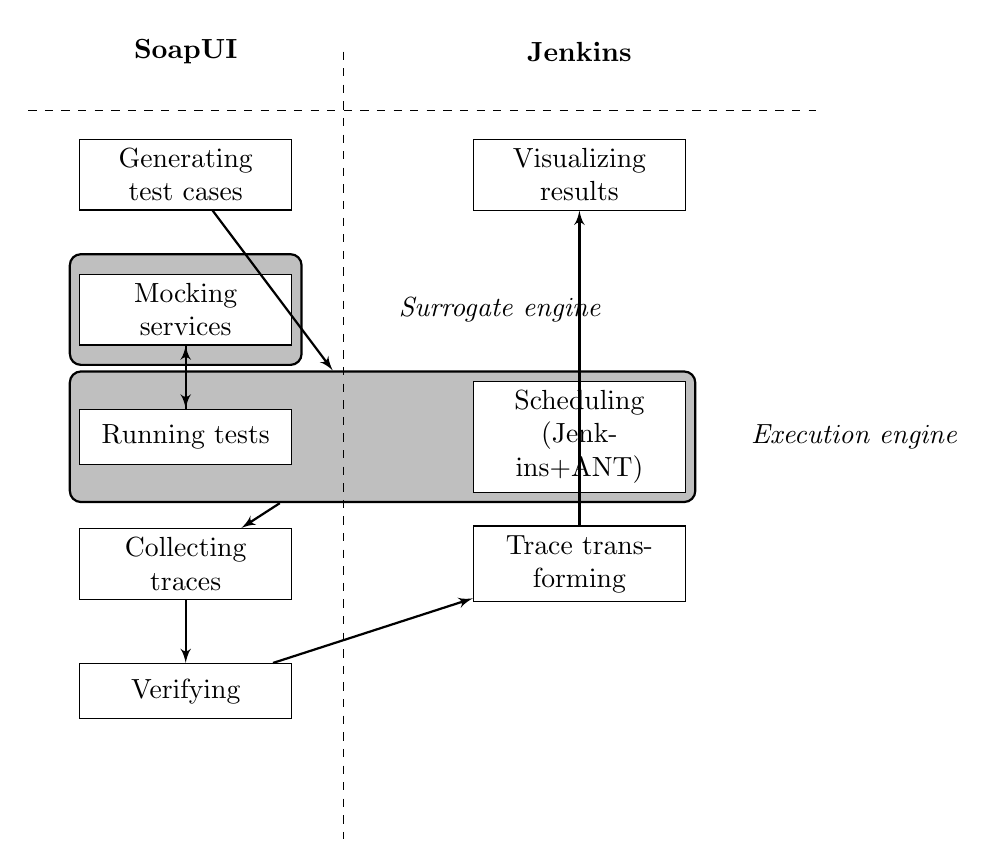
\begin{tikzpicture}[
    start chain=going below,    % General flow is top-to-bottom
    node distance=8mm and 50mm, % Global setup of box spacing
    ]
% ------------------------------------------------- 
\tikzset{
  base/.style={draw, on chain, on grid, align=center, minimum height=4ex},
  label/.style={on chain, on grid, align=center, minimum height=4ex},
  proc/.style={base, rectangle, minimum height=2em, text width=7em, fill=white},
  box/.style={draw, thick, minimum height=4em, fill=lightgray, rectangle, rounded corners},
  line/.style={draw, thick, -latex'}
}
% -------------------------------------------------
% Placing the nodes

\draw [dashed] (2,0) -- (2,-10);
\draw [dashed] (-2,-0.75) -- (8,-0.75);
\node[label] (l0) {\textbf{SoapUI}};

\node [proc] (p0) {Generating test cases};
\node [proc] (p1) {Mocking services};
\node [proc] (p2) {Running tests};
\node [proc] (p3) {Collecting traces};
\node [proc] (p4) {Verifying};

\node[label, right=of l0] (l1) {\textbf{Jenkins}};
\node [proc, right=of p2] (p5) {Scheduling (Jenkins+ANT)};
\node [proc, right=of p3] (p6) {Trace transforming};

\node [proc, right=of p0] (p7) {Visualizing results};

\begin{pgfonlayer}{background}
  \node[box] [fit = (p2) (p5)] (b0) {}; % Execution engine
\end{pgfonlayer}

\begin{pgfonlayer}{background}
  \node[box] [fit = (p1)] (b1) {};      % Surrogate engine
\end{pgfonlayer}

\node[label, right=3.5cm of p5] {\emph{Execution engine}};
\node[label, right=4cm of p1] {\emph{Surrogate engine}};

\path [line] (p0) -- (b0);
\path [line] (p2) -- (p1);
\path [line] (p1) -- (p2);
\path [line] (b0) -- (p3);
\path [line] (p3) -- (p4);
\path [line] (p4) -- (p6);
\path [line] (p6) -- (p7);

\end{tikzpicture}
\caption{Testing framework structure} \label{fig:structure}
\end{figure}

In the framework architecture, SoapUI contains script logic and in MVC terms acts as model, while Jenkins provides a user interface for control and view. The experiment quickly showed the difficulty of dividing responsibility between software components. Implementing a feature like test execution requires cooperation between tools where one assumes part of the duties while the other fulfills the rest. Depending on the observers perspective either in true irony --- or an illustrative example --- implementing the integration testing framework already creates a number of system dependencies.

Execution engine duties are split between the actual running of the tests and scheduling test cycles. The execution engine running the tests, SoapUI, also collects execution traces. These are transformed into legible form (simple text) and can be examined in the Jenkins UI. Accordingly, what can only be called a gross initial oversight, visualizing the test results is added as a process to the overall framework process.

\subsection{SoapUI}

\textbf{SoapUI}\footnote{http://www.soapui.org} is an IDE, or integrated development environment, and is used in constructing test scripts, both manually and through \emph{capture and playback}. Capture can also be used to to create scripts to simulate the behavior of systems thereby satisfying the requirement of having surrogate engines. Effectively, SoapUI uses capture for both test case \emph{and surrogate engine} generation. These mock service surrogates allow verification by providing an otherwise absent execution trail or returning courtesy messages of the test outcome, or what has happened across the integration black box.

After their creation test cases can be run in SoapUI and the tool affords a program script that can be run on the command line simply by specifying which SoapUI project and which test suite or cases should be run.

Because specification of sufficient accuracy for deriving test cases automatically were not available, test cases are based on capture. Test cases are written in a SoapUI-tailored template format but since their structural composition is largely that of an XML file, their fair reusability and low risk of vendor lock-in is justified. 

Execution traces are simply full text accounts of test results. These include information on the test case level or which case failed, which is why tests should only have one assertion if possible as this helps seeing what exactly is wrong the program and where the defect might be \citep{duvall2007continuous}.

\subsection{Jenkins}

\textbf{Jenkins}\footnote{http://jenkins-ci.org/} is a continuous testing and integration tool which manages test execution for software projects. Running on a server, Jenkins can be triggered to run on a regular basis (e.g. daily, weekly, every hour) or immediately as new code is committed into a repository linked to a Jenkins project. Since test cases, suites, collections of suites can be linked to independent projects, it is easy to organize tests, tailor and schedule runs, and generally execute tests only when it is needed\footnote{A Jenkins project may be rigged to run any number of test suites which in turn can contain any number test cases. Projects can therefore be configured to test an area or areas of functionality --- or perform all tests.}.

It should be noted that Jenkins is made with software development rather than regression testing in mind but on balance the regression test set-up is equally effective. At the bare minimum, Jenkins is given a test case execution script courtesy of SoapUI which it runs in the native operating system's environment and collects traces provided by the cases and script.

Jenkins is used in conjunction with ANT, which while not necessary, is an industry best practice and contains advantages cross-system configuration. ANT is essentially an XML-format configuration file which specifies which steps are to be taken when a new build, i.e. updated version, is created. The build can be appended with software engineering tasks, including running a test execution script. 

% muokka database kohta, ei ole laukkaen mallissa
% lisää kuva project - suite - case suhteesta?

\subsection{Heuristic evaluation of the framework}

The framework is evaluated mainly by qualitative measures, but a quick heuristic analysis is also used to validate to new model. This done by comparisons to the idealized models, testing theory, and recommendations from integration experts.

Compared to the models by \citet{liu2009unified} and \citet{huang2008surrogate} in Chapter \ref{chapter:frameworktheory} the new model covers most the same ground with the addition of the surrogate generation process. 
% Platform independennce not requirement for Wärtsilä, involved coding plugins and adapters, which should be avoiuded

\citeauthor{laukkanen2006data}'s \citeyearpar{laukkanen2006data} framework includes test asset management as a responsibility area to control test cases and attached data. The framework could be extended with a database to manage test resources.

\citet{fewster1999software} present key characteristics of an automated regime test regime, a system of government of testing which can be likened to a framework but with more emphasis on governance and rules of practice. Characteristics of a good test regime are:
\begin{itemize}
\item easy to select tests to be run at the touch of a button
\item tests take care of all their housekeeping such as environmental set-up and clear-down
\item it is easier to add a new test to the automated pack than to run that test manually
\end{itemize}

The framework satisfies the first criteria easily. Executing packages of tests packages in Jenkins is done with a simple click. Likewise choosing which tests to execute is not uncomplicated. Integration test cases can be organised inside Jenkins projects so that only the needed cases are run. This does call for some maintenance work, however. It is essential to know which projects should be appended with the new case. Otherwise the unorganized collection test cases becomes clumsy to use. This issue can be subverted by guidelines already at the test creation process so that the test engineer adds the case in the correct test suite. The framework administrator meanwhile sees to that each suite is correctly linked to projects.

Automated testing already requires the second criteria be satisfied. Assuming the test server and SUT servers are available, and test cases contain necessary information to access information services, the test set-up is complete. Because some features require inputting information, like creating test orders, which can not be allowed in production, mock services are used. Here, test messages travel through the same \emph{"integration black box"} as actual messages would, and the only part that is not "real" is the end point system the testing of which is outside of integration test scope. Therefore the described test approach provides an accurate result of integration functionality and health. Not part of the automation, a test engineer should monitor execution and react appropriately in case a test case fails.

As for the third criterion, running a test manually and adding the test to the automated pack both require writing or generating the case first. With a good template and guidelines in place, the case writing task can be expedited and the engineer adds the case to the correct suite where it will automatically be picked up by the test scripts run through the framework.

\section{Qualitative evaluation}

% should there be more requirements in the background section, add interviews summarize succinctly
Qualitative evaluation of the new framework is performed through interviews with Wärtsilä's experts in a workshop, and observations of the framework in simulated action.

% should there be interviews about what is wrong with testing now
% ville: health check
% paavo: 
% eero: protocols, requirements
% why interviewees slected

\subsection{Workshop}

A workshop was organized to showcase the new framework model to interested parties inside Wärtsilä and to evaluate its applicability in the company. The purpose of the event was twofold: to validate and improve. Feedback both critical and supportive was elicited and suggestions for further improvement collected. The workshop event was facilitated by the author.

Of particular interest are the observations of people who're actually to use the framework if it were adopted. How do they see creating test cases, managing test results, or otherwise maintaining the framework. 

what it requires from people, integration managers create test cases in own project, updates, responsibility
who packages suites?

The workshop was recorded. In the session everyone was given a presentation and demo of the the framework after which everyone was given a chance to voice their first impressions. The workshop was facilitated by the researcher asking questions when necessary to kick-start discussion or move it to a new topic.


% All the discussion was taped and the participants were given Post-it notes to write down all ideas that surfaced during the workshop. In total six persons - consisting of developers from maintenance, team leaders and one senior manager - attended the workshop.
% Goals - applicability of the model, questioning it
% validate and improve

% teknisempi kuvaus? kenellä on nyt integraatiovastuu ja kuka testaa 
% research method

\chapter{Evaluation}
\label{chapter:evaluation}

who will create test cases. which tool is easiest to use and most feasible.

\section{Evaluation of the empirical experiment and revised prototype framework}

\chapter{Discussion}
\label{chapter:discussion}

One of the fundamental difficulties in developing an integration testing framework is the intertwined relationship of technology and manual work involved in and around it. Clearly as a framework for \emph{automated} testing the framework is realized by algorithmical execution, but it cannot be used successfully without human intervention and maintenance. It is blurred relationship of man and machine, the concoction of technological configuration and human work process model tries the framework developer.

Future research:
capture playback popular still despite warnings, what's up? when is it not applicable?
relationship between automation and manual work, test automation manual maintenance
integration test strategy in the vein if rehmann, what options/technical strategies are there? tired old big-bang
Strategies for test case creation (zeng & tan 2013)
study merits of fault based testing for more efficient tests
distinction between a technological configuration and process model is difficult.

notion of unit to system antiquated, block to block also
more an issue of test case construction and traceability
end-to-end tests are adequate if they can point to problem code accurately

\chapter{Conclusions}
\label{chapter:conclusions}

It is not possible to go through every code branch or to test every possible input sequence. As \citet{myers1976software} put it, testing is a problem in economics. Test cases must provide a maximum yield on investment, where yield is measured as the probability that the case uncovers a new defect. \citep{myers1976software} 

Good planning is required and ensured by good governance and realized by a well-documented process model and carried out in practice by a technological framework. The strategy-operation alignment process goes through many gates and finding the right fit is not easy.

could benefit any company doing testing based on capture replay, focusing on testing integrations. the process defined.

\begin{comment}
% pezze integration faults
Inconsistent interpretation of parameters or values
Violations of value domains or of capacity or size limits
Side-effects on parameters or resrouces
Missing or misunderstood functionality
Nonfinctional problems
Dynamic mismatches
\end{comment}

\begin{comment}
Interpretation
    wrong function - something else than specified
    extra function - more than what is expected/needed
    missing function - not all that is specified
Miscoded call (error which causes the developer to place the call instruction at the wrong point in the program)
    Extra instruction fault: the call instruction is on a path which should not have the call.
    Wrong placement fault: the call is at the wrong location on the path which should have the call instruction.
    Missing instruction fault: the call instruction is missing on the path which should have the call.
Interface error
    When stardards or agreements are violated
\end{comment}

% ERRORS: wrong function, extra function, missing function 
% Miscoded call error
% Interface error (Lueng \& white)
% =================================================

% Thin threads, groupin into a tree (tsai et al)
% Test data difficult to select (linnenkugel mullburg)
% add background informtion: general about regression/integration/software testing, ITIL processes at Wärtsilä
% and possibly more...
% Todo: add Harness as testing strategy

% Load the bibliographic references
% ------------------------------------------------------------------
% You can use several .bib files:
% \bibliography{thesis_sources,ietf_sources}
\bibliography{ref}

% Appendices go here
% ------------------------------------------------------------------
% If you do not have appendices, comment out the following lines
\appendix
% \input{appendices.tex}

\chapter{First appendix}
\label{chapter:first-appendix}

This is the first appendix. You could put some test images or verbose data in an
appendix, if there is too much data to fit in the actual text nicely.

For now, the Aalto logo variants are shown in Figure~\ref{fig:aaltologo}.

\begin{figure}
\begin{center}
\subfigure[In English]{\includegraphics[width=.8\textwidth]{aalto-logo-en}}
\subfigure[Suomeksi]{\includegraphics[width=.8\textwidth]{aalto-logo-fi}}
\subfigure[Pä svenska]{\includegraphics[width=.8\textwidth]{aalto-logo-se}}
\caption{Aalto logo variants}
\label{fig:aaltologo}
\end{center}
\end{figure}

% End of document!
% ------------------------------------------------------------------
% The LastPage package automatically places a label on the last page.
% That works better than placing a label here manually, because the
% label might not go to the actual last page, if LaTeX needs to place
% floats (that is, figures, tables, and such) to the end of the
% document.
\end{document}